\documentclass[twoside]{book}

% Packages required by doxygen
\usepackage{fixltx2e}
\usepackage{calc}
\usepackage{doxygen}
\usepackage[export]{adjustbox} % also loads graphicx
\usepackage{graphicx}
\usepackage[utf8]{inputenc}
\usepackage{makeidx}
\usepackage{multicol}
\usepackage{multirow}
\PassOptionsToPackage{warn}{textcomp}
\usepackage{textcomp}
\usepackage[nointegrals]{wasysym}
\usepackage[table]{xcolor}

% Font selection
\usepackage[T1]{fontenc}
\usepackage[scaled=.90]{helvet}
\usepackage{courier}
\usepackage{amssymb}
\usepackage{sectsty}
\renewcommand{\familydefault}{\sfdefault}
\allsectionsfont{%
  \fontseries{bc}\selectfont%
  \color{darkgray}%
}
\renewcommand{\DoxyLabelFont}{%
  \fontseries{bc}\selectfont%
  \color{darkgray}%
}
\newcommand{\+}{\discretionary{\mbox{\scriptsize$\hookleftarrow$}}{}{}}

% Page & text layout
\usepackage{geometry}
\geometry{%
  a4paper,%
  top=2.5cm,%
  bottom=2.5cm,%
  left=2.5cm,%
  right=2.5cm%
}
\tolerance=750
\hfuzz=15pt
\hbadness=750
\setlength{\emergencystretch}{15pt}
\setlength{\parindent}{0cm}
\setlength{\parskip}{3ex plus 2ex minus 2ex}
\makeatletter
\renewcommand{\paragraph}{%
  \@startsection{paragraph}{4}{0ex}{-1.0ex}{1.0ex}{%
    \normalfont\normalsize\bfseries\SS@parafont%
  }%
}
\renewcommand{\subparagraph}{%
  \@startsection{subparagraph}{5}{0ex}{-1.0ex}{1.0ex}{%
    \normalfont\normalsize\bfseries\SS@subparafont%
  }%
}
\makeatother

% Headers & footers
\usepackage{fancyhdr}
\pagestyle{fancyplain}
\fancyhead[LE]{\fancyplain{}{\bfseries\thepage}}
\fancyhead[CE]{\fancyplain{}{}}
\fancyhead[RE]{\fancyplain{}{\bfseries\leftmark}}
\fancyhead[LO]{\fancyplain{}{\bfseries\rightmark}}
\fancyhead[CO]{\fancyplain{}{}}
\fancyhead[RO]{\fancyplain{}{\bfseries\thepage}}
\fancyfoot[LE]{\fancyplain{}{}}
\fancyfoot[CE]{\fancyplain{}{}}
\fancyfoot[RE]{\fancyplain{}{\bfseries\scriptsize Generated by Doxygen }}
\fancyfoot[LO]{\fancyplain{}{\bfseries\scriptsize Generated by Doxygen }}
\fancyfoot[CO]{\fancyplain{}{}}
\fancyfoot[RO]{\fancyplain{}{}}
\renewcommand{\footrulewidth}{0.4pt}
\renewcommand{\chaptermark}[1]{%
  \markboth{#1}{}%
}
\renewcommand{\sectionmark}[1]{%
  \markright{\thesection\ #1}%
}

% Indices & bibliography
\usepackage{natbib}
\usepackage[titles]{tocloft}
\setcounter{tocdepth}{3}
\setcounter{secnumdepth}{5}
\makeindex

% Hyperlinks (required, but should be loaded last)
\usepackage{ifpdf}
\ifpdf
  \usepackage[pdftex,pagebackref=true]{hyperref}
\else
  \usepackage[ps2pdf,pagebackref=true]{hyperref}
\fi
\hypersetup{%
  colorlinks=true,%
  linkcolor=blue,%
  citecolor=blue,%
  unicode%
}

% Custom commands
\newcommand{\clearemptydoublepage}{%
  \newpage{\pagestyle{empty}\cleardoublepage}%
}

\usepackage{caption}
\captionsetup{labelsep=space,justification=centering,font={bf},singlelinecheck=off,skip=4pt,position=top}

%===== C O N T E N T S =====

\begin{document}

% Titlepage & ToC
\hypersetup{pageanchor=false,
             bookmarksnumbered=true,
             pdfencoding=unicode
            }
\pagenumbering{alph}
\begin{titlepage}
\vspace*{7cm}
\begin{center}%
{\Large c++ library collection }\\
\vspace*{1cm}
{\large Generated by Doxygen 1.8.13}\\
\end{center}
\end{titlepage}
\clearemptydoublepage
\pagenumbering{roman}
\tableofcontents
\clearemptydoublepage
\pagenumbering{arabic}
\hypersetup{pageanchor=true}

%--- Begin generated contents ---
\chapter{Cpp\+Libs}
\label{md_README}
\Hypertarget{md_README}
\subsection*{T\+O\+DO}


\begin{DoxyItemize}
\item input stream and output stream separate closable (?)
\end{DoxyItemize}

\subsection*{Build}

run ./configure make -\/C build

\subsection*{Documentation}

available\+: \href{https://devfix.github.io/cpplibs/html/index.html}{\tt here} 
\chapter{Namespace Index}
\section{Namespace List}
Here is a list of all namespaces with brief descriptions\+:\begin{DoxyCompactList}
\item\contentsline{section}{\hyperlink{namespacedevfix}{devfix} }{\pageref{namespacedevfix}}{}
\item\contentsline{section}{\hyperlink{namespacedevfix_1_1base}{devfix\+::base} \\*Root namespace of devfix base library }{\pageref{namespacedevfix_1_1base}}{}
\item\contentsline{section}{\hyperlink{namespacedevfix_1_1base_1_1__math}{devfix\+::base\+::\+\_\+math} }{\pageref{namespacedevfix_1_1base_1_1__math}}{}
\item\contentsline{section}{\hyperlink{namespacedevfix_1_1base_1_1error}{devfix\+::base\+::error} \\*Namespace for general errors like timeouts or io failures }{\pageref{namespacedevfix_1_1base_1_1error}}{}
\item\contentsline{section}{\hyperlink{namespacedevfix_1_1base_1_1io}{devfix\+::base\+::io} \\*Namespace for io tool, for instance streams }{\pageref{namespacedevfix_1_1base_1_1io}}{}
\item\contentsline{section}{\hyperlink{namespacedevfix_1_1base_1_1numbers}{devfix\+::base\+::numbers} }{\pageref{namespacedevfix_1_1base_1_1numbers}}{}
\item\contentsline{section}{\hyperlink{namespacedevfix_1_1dsp}{devfix\+::dsp} }{\pageref{namespacedevfix_1_1dsp}}{}
\item\contentsline{section}{\hyperlink{namespacedevfix_1_1net}{devfix\+::net} \\*Root namespace of devfix network library }{\pageref{namespacedevfix_1_1net}}{}
\end{DoxyCompactList}

\chapter{Hierarchical Index}
\section{Class Hierarchy}
This inheritance list is sorted roughly, but not completely, alphabetically\+:\begin{DoxyCompactList}
\item exception\begin{DoxyCompactList}
\item \contentsline{section}{devfix\+:\+:base\+:\+:error\+:\+:baseexception}{\pageref{structdevfix_1_1base_1_1error_1_1baseexception}}{}
\begin{DoxyCompactList}
\item \contentsline{section}{devfix\+:\+:base\+:\+:error\+:\+:interruptedexception}{\pageref{structdevfix_1_1base_1_1error_1_1interruptedexception}}{}
\item \contentsline{section}{devfix\+:\+:base\+:\+:error\+:\+:ioexception}{\pageref{structdevfix_1_1base_1_1error_1_1ioexception}}{}
\item \contentsline{section}{devfix\+:\+:base\+:\+:error\+:\+:timeoutexception}{\pageref{structdevfix_1_1base_1_1error_1_1timeoutexception}}{}
\item \contentsline{section}{devfix\+:\+:net\+:\+:socketexception}{\pageref{structdevfix_1_1net_1_1socketexception}}{}
\end{DoxyCompactList}
\end{DoxyCompactList}
\item \contentsline{section}{devfix\+:\+:net\+:\+:inetaddress}{\pageref{structdevfix_1_1net_1_1inetaddress}}{}
\item \contentsline{section}{devfix\+:\+:base\+:\+:io\+:\+:inputstream}{\pageref{structdevfix_1_1base_1_1io_1_1inputstream}}{}
\begin{DoxyCompactList}
\item \contentsline{section}{devfix\+:\+:base\+:\+:io\+:\+:source}{\pageref{structdevfix_1_1base_1_1io_1_1source}}{}
\end{DoxyCompactList}
\item \contentsline{section}{devfix\+:\+:net\+:\+:netbuilder}{\pageref{structdevfix_1_1net_1_1netbuilder}}{}
\item \contentsline{section}{devfix\+:\+:base\+:\+:io\+:\+:outputstream}{\pageref{structdevfix_1_1base_1_1io_1_1outputstream}}{}
\begin{DoxyCompactList}
\item \contentsline{section}{devfix\+:\+:base\+:\+:io\+:\+:sink}{\pageref{structdevfix_1_1base_1_1io_1_1sink}}{}
\end{DoxyCompactList}
\item \contentsline{section}{devfix\+:\+:net\+:\+:serversocket}{\pageref{structdevfix_1_1net_1_1serversocket}}{}
\item \contentsline{section}{devfix\+:\+:net\+:\+:socket}{\pageref{structdevfix_1_1net_1_1socket}}{}
\end{DoxyCompactList}

\chapter{Class Index}
\section{Class List}
Here are the classes, structs, unions and interfaces with brief descriptions\+:\begin{DoxyCompactList}
\item\contentsline{section}{\hyperlink{structdevfix_1_1base_1_1error_1_1baseexception}{devfix\+::base\+::error\+::baseexception} \\*Abstract error base class }{\pageref{structdevfix_1_1base_1_1error_1_1baseexception}}{}
\item\contentsline{section}{\hyperlink{structdevfix_1_1net_1_1inetaddress}{devfix\+::net\+::inetaddress} }{\pageref{structdevfix_1_1net_1_1inetaddress}}{}
\item\contentsline{section}{\hyperlink{structdevfix_1_1base_1_1io_1_1inputstream}{devfix\+::base\+::io\+::inputstream} \\*Superclass of all classes representing an input stream of bytes }{\pageref{structdevfix_1_1base_1_1io_1_1inputstream}}{}
\item\contentsline{section}{\hyperlink{structdevfix_1_1base_1_1error_1_1interruptedexception}{devfix\+::base\+::error\+::interruptedexception} \\*Thrown when an operation is interrupted, either before or during the activity }{\pageref{structdevfix_1_1base_1_1error_1_1interruptedexception}}{}
\item\contentsline{section}{\hyperlink{structdevfix_1_1base_1_1error_1_1ioexception}{devfix\+::base\+::error\+::ioexception} \\*Signals that an I/O error of some sort has occurred }{\pageref{structdevfix_1_1base_1_1error_1_1ioexception}}{}
\item\contentsline{section}{\hyperlink{structdevfix_1_1net_1_1netbuilder}{devfix\+::net\+::netbuilder} }{\pageref{structdevfix_1_1net_1_1netbuilder}}{}
\item\contentsline{section}{\hyperlink{structdevfix_1_1base_1_1io_1_1outputstream}{devfix\+::base\+::io\+::outputstream} \\*Superclass of all classes representing an output stream of bytes }{\pageref{structdevfix_1_1base_1_1io_1_1outputstream}}{}
\item\contentsline{section}{\hyperlink{structdevfix_1_1net_1_1serversocket}{devfix\+::net\+::serversocket} }{\pageref{structdevfix_1_1net_1_1serversocket}}{}
\item\contentsline{section}{\hyperlink{structdevfix_1_1base_1_1io_1_1sink}{devfix\+::base\+::io\+::sink} }{\pageref{structdevfix_1_1base_1_1io_1_1sink}}{}
\item\contentsline{section}{\hyperlink{structdevfix_1_1net_1_1socket}{devfix\+::net\+::socket} }{\pageref{structdevfix_1_1net_1_1socket}}{}
\item\contentsline{section}{\hyperlink{structdevfix_1_1net_1_1socketexception}{devfix\+::net\+::socketexception} \\*Thrown to indicate that there is an error creating or accessing a Socket }{\pageref{structdevfix_1_1net_1_1socketexception}}{}
\item\contentsline{section}{\hyperlink{structdevfix_1_1base_1_1io_1_1source}{devfix\+::base\+::io\+::source} }{\pageref{structdevfix_1_1base_1_1io_1_1source}}{}
\item\contentsline{section}{\hyperlink{structdevfix_1_1base_1_1error_1_1timeoutexception}{devfix\+::base\+::error\+::timeoutexception} \\*Exception thrown when a blocking operation times out }{\pageref{structdevfix_1_1base_1_1error_1_1timeoutexception}}{}
\end{DoxyCompactList}

\chapter{Namespace Documentation}
\hypertarget{namespacedevfix_1_1base_1_1error}{}\section{devfix\+:\+:base\+:\+:error Namespace Reference}
\label{namespacedevfix_1_1base_1_1error}\index{devfix\+::base\+::error@{devfix\+::base\+::error}}


Namespace for general errors like timeouts or io failures.  


\subsection*{Classes}
\begin{DoxyCompactItemize}
\item 
struct \hyperlink{structdevfix_1_1base_1_1error_1_1baseexception}{baseexception}
\begin{DoxyCompactList}\small\item\em Abstract error base class. \end{DoxyCompactList}\item 
struct \hyperlink{structdevfix_1_1base_1_1error_1_1interruptedexception}{interruptedexception}
\begin{DoxyCompactList}\small\item\em Thrown when an operation is interrupted, either before or during the activity. \end{DoxyCompactList}\item 
struct \hyperlink{structdevfix_1_1base_1_1error_1_1ioexception}{ioexception}
\begin{DoxyCompactList}\small\item\em Signals that an I/O error of some sort has occurred. \end{DoxyCompactList}\item 
struct \hyperlink{structdevfix_1_1base_1_1error_1_1timeoutexception}{timeoutexception}
\begin{DoxyCompactList}\small\item\em Exception thrown when a blocking operation times out. \end{DoxyCompactList}\end{DoxyCompactItemize}


\subsection{Detailed Description}
Namespace for general errors like timeouts or io failures. 

More specific exceptions are in the namespace of their corresponding functionality. 
\hypertarget{namespacedevfix_1_1base_1_1io}{}\section{devfix\+:\+:base\+:\+:io Namespace Reference}
\label{namespacedevfix_1_1base_1_1io}\index{devfix\+::base\+::io@{devfix\+::base\+::io}}


Namespace for io tool, for instance streams.  


\subsection*{Classes}
\begin{DoxyCompactItemize}
\item 
struct \hyperlink{structdevfix_1_1base_1_1io_1_1inputstream}{inputstream}
\begin{DoxyCompactList}\small\item\em Superclass of all classes representing an input stream of bytes. \end{DoxyCompactList}\item 
struct \hyperlink{structdevfix_1_1base_1_1io_1_1outputstream}{outputstream}
\begin{DoxyCompactList}\small\item\em Superclass of all classes representing an output stream of bytes. \end{DoxyCompactList}\item 
struct \hyperlink{structdevfix_1_1base_1_1io_1_1sink}{sink}
\item 
struct \hyperlink{structdevfix_1_1base_1_1io_1_1source}{source}
\end{DoxyCompactItemize}
\subsection*{Typedefs}
\begin{DoxyCompactItemize}
\item 
typedef std\+::function$<$ void()$>$ \hyperlink{namespacedevfix_1_1base_1_1io_ae3118387742e5f4d484a328a213d6a5d}{close\+\_\+t}
\item 
typedef std\+::function$<$ bool()$>$ \hyperlink{namespacedevfix_1_1base_1_1io_a14f89d4437ced6ede49c044ee8e71f17}{is\+\_\+closed\+\_\+t}
\item 
typedef std\+::function$<$ void(void $\ast$, std\+::size\+\_\+t)$>$ \hyperlink{namespacedevfix_1_1base_1_1io_afa65222ee5a1636be18df5e16bbcf858}{read\+\_\+t}
\item 
typedef std\+::function$<$ void(std\+::size\+\_\+t)$>$ \hyperlink{namespacedevfix_1_1base_1_1io_aeb8f94d85cfeaa405f53a6967e609645}{skip\+\_\+t}
\item 
typedef std\+::function$<$ std\+::size\+\_\+t()$>$ \hyperlink{namespacedevfix_1_1base_1_1io_a19c1195ab6a44e6d4f48b86062860a11}{available\+\_\+t}
\item 
typedef std\+::function$<$ void(const void $\ast$, std\+::size\+\_\+t)$>$ \hyperlink{namespacedevfix_1_1base_1_1io_a75953e4d7f81d76e419f9672ffedda87}{write\+\_\+t}
\item 
typedef std\+::function$<$ void()$>$ \hyperlink{namespacedevfix_1_1base_1_1io_a622685976c7f503411827fba028d3ce1}{flush\+\_\+t}
\end{DoxyCompactItemize}
\subsection*{Variables}
\begin{DoxyCompactItemize}
\item 
const \hyperlink{namespacedevfix_1_1base_1_1io_ae3118387742e5f4d484a328a213d6a5d}{close\+\_\+t} \hyperlink{namespacedevfix_1_1base_1_1io_a14a286c17d4b93881d42b1d14beb2d0b}{D\+E\+F\+A\+U\+L\+T\+\_\+\+C\+L\+O\+SE} = \mbox{[}$\,$\mbox{]}() \{\}
\item 
const \hyperlink{namespacedevfix_1_1base_1_1io_a14f89d4437ced6ede49c044ee8e71f17}{is\+\_\+closed\+\_\+t} \hyperlink{namespacedevfix_1_1base_1_1io_ae04fec2a2a2db3482e624a59e59a2a14}{D\+E\+F\+A\+U\+L\+T\+\_\+\+I\+S\+\_\+\+C\+L\+O\+S\+ED} = \mbox{[}$\,$\mbox{]}() \{ return false; \}
\end{DoxyCompactItemize}


\subsection{Detailed Description}
Namespace for io tool, for instance streams. 

\subsection{Typedef Documentation}
\mbox{\Hypertarget{namespacedevfix_1_1base_1_1io_a19c1195ab6a44e6d4f48b86062860a11}\label{namespacedevfix_1_1base_1_1io_a19c1195ab6a44e6d4f48b86062860a11}} 
\index{devfix\+::base\+::io@{devfix\+::base\+::io}!available\+\_\+t@{available\+\_\+t}}
\index{available\+\_\+t@{available\+\_\+t}!devfix\+::base\+::io@{devfix\+::base\+::io}}
\subsubsection{\texorpdfstring{available\+\_\+t}{available\_t}}
{\footnotesize\ttfamily typedef std\+::function$<$std\+::size\+\_\+t()$>$ \hyperlink{namespacedevfix_1_1base_1_1io_a19c1195ab6a44e6d4f48b86062860a11}{devfix\+::base\+::io\+::available\+\_\+t}}

\mbox{\Hypertarget{namespacedevfix_1_1base_1_1io_ae3118387742e5f4d484a328a213d6a5d}\label{namespacedevfix_1_1base_1_1io_ae3118387742e5f4d484a328a213d6a5d}} 
\index{devfix\+::base\+::io@{devfix\+::base\+::io}!close\+\_\+t@{close\+\_\+t}}
\index{close\+\_\+t@{close\+\_\+t}!devfix\+::base\+::io@{devfix\+::base\+::io}}
\subsubsection{\texorpdfstring{close\+\_\+t}{close\_t}}
{\footnotesize\ttfamily typedef std\+::function$<$void()$>$ \hyperlink{namespacedevfix_1_1base_1_1io_ae3118387742e5f4d484a328a213d6a5d}{devfix\+::base\+::io\+::close\+\_\+t}}

\mbox{\Hypertarget{namespacedevfix_1_1base_1_1io_a622685976c7f503411827fba028d3ce1}\label{namespacedevfix_1_1base_1_1io_a622685976c7f503411827fba028d3ce1}} 
\index{devfix\+::base\+::io@{devfix\+::base\+::io}!flush\+\_\+t@{flush\+\_\+t}}
\index{flush\+\_\+t@{flush\+\_\+t}!devfix\+::base\+::io@{devfix\+::base\+::io}}
\subsubsection{\texorpdfstring{flush\+\_\+t}{flush\_t}}
{\footnotesize\ttfamily typedef std\+::function$<$void()$>$ \hyperlink{namespacedevfix_1_1base_1_1io_a622685976c7f503411827fba028d3ce1}{devfix\+::base\+::io\+::flush\+\_\+t}}

\mbox{\Hypertarget{namespacedevfix_1_1base_1_1io_a14f89d4437ced6ede49c044ee8e71f17}\label{namespacedevfix_1_1base_1_1io_a14f89d4437ced6ede49c044ee8e71f17}} 
\index{devfix\+::base\+::io@{devfix\+::base\+::io}!is\+\_\+closed\+\_\+t@{is\+\_\+closed\+\_\+t}}
\index{is\+\_\+closed\+\_\+t@{is\+\_\+closed\+\_\+t}!devfix\+::base\+::io@{devfix\+::base\+::io}}
\subsubsection{\texorpdfstring{is\+\_\+closed\+\_\+t}{is\_closed\_t}}
{\footnotesize\ttfamily typedef std\+::function$<$bool()$>$ \hyperlink{namespacedevfix_1_1base_1_1io_a14f89d4437ced6ede49c044ee8e71f17}{devfix\+::base\+::io\+::is\+\_\+closed\+\_\+t}}

\mbox{\Hypertarget{namespacedevfix_1_1base_1_1io_afa65222ee5a1636be18df5e16bbcf858}\label{namespacedevfix_1_1base_1_1io_afa65222ee5a1636be18df5e16bbcf858}} 
\index{devfix\+::base\+::io@{devfix\+::base\+::io}!read\+\_\+t@{read\+\_\+t}}
\index{read\+\_\+t@{read\+\_\+t}!devfix\+::base\+::io@{devfix\+::base\+::io}}
\subsubsection{\texorpdfstring{read\+\_\+t}{read\_t}}
{\footnotesize\ttfamily typedef std\+::function$<$void(void $\ast$, std\+::size\+\_\+t)$>$ \hyperlink{namespacedevfix_1_1base_1_1io_afa65222ee5a1636be18df5e16bbcf858}{devfix\+::base\+::io\+::read\+\_\+t}}

\mbox{\Hypertarget{namespacedevfix_1_1base_1_1io_aeb8f94d85cfeaa405f53a6967e609645}\label{namespacedevfix_1_1base_1_1io_aeb8f94d85cfeaa405f53a6967e609645}} 
\index{devfix\+::base\+::io@{devfix\+::base\+::io}!skip\+\_\+t@{skip\+\_\+t}}
\index{skip\+\_\+t@{skip\+\_\+t}!devfix\+::base\+::io@{devfix\+::base\+::io}}
\subsubsection{\texorpdfstring{skip\+\_\+t}{skip\_t}}
{\footnotesize\ttfamily typedef std\+::function$<$void(std\+::size\+\_\+t)$>$ \hyperlink{namespacedevfix_1_1base_1_1io_aeb8f94d85cfeaa405f53a6967e609645}{devfix\+::base\+::io\+::skip\+\_\+t}}

\mbox{\Hypertarget{namespacedevfix_1_1base_1_1io_a75953e4d7f81d76e419f9672ffedda87}\label{namespacedevfix_1_1base_1_1io_a75953e4d7f81d76e419f9672ffedda87}} 
\index{devfix\+::base\+::io@{devfix\+::base\+::io}!write\+\_\+t@{write\+\_\+t}}
\index{write\+\_\+t@{write\+\_\+t}!devfix\+::base\+::io@{devfix\+::base\+::io}}
\subsubsection{\texorpdfstring{write\+\_\+t}{write\_t}}
{\footnotesize\ttfamily typedef std\+::function$<$void(const void $\ast$, std\+::size\+\_\+t)$>$ \hyperlink{namespacedevfix_1_1base_1_1io_a75953e4d7f81d76e419f9672ffedda87}{devfix\+::base\+::io\+::write\+\_\+t}}



\subsection{Variable Documentation}
\mbox{\Hypertarget{namespacedevfix_1_1base_1_1io_a14a286c17d4b93881d42b1d14beb2d0b}\label{namespacedevfix_1_1base_1_1io_a14a286c17d4b93881d42b1d14beb2d0b}} 
\index{devfix\+::base\+::io@{devfix\+::base\+::io}!D\+E\+F\+A\+U\+L\+T\+\_\+\+C\+L\+O\+SE@{D\+E\+F\+A\+U\+L\+T\+\_\+\+C\+L\+O\+SE}}
\index{D\+E\+F\+A\+U\+L\+T\+\_\+\+C\+L\+O\+SE@{D\+E\+F\+A\+U\+L\+T\+\_\+\+C\+L\+O\+SE}!devfix\+::base\+::io@{devfix\+::base\+::io}}
\subsubsection{\texorpdfstring{D\+E\+F\+A\+U\+L\+T\+\_\+\+C\+L\+O\+SE}{DEFAULT\_CLOSE}}
{\footnotesize\ttfamily const \hyperlink{namespacedevfix_1_1base_1_1io_ae3118387742e5f4d484a328a213d6a5d}{close\+\_\+t} devfix\+::base\+::io\+::\+D\+E\+F\+A\+U\+L\+T\+\_\+\+C\+L\+O\+SE = \mbox{[}$\,$\mbox{]}() \{\}}

\mbox{\Hypertarget{namespacedevfix_1_1base_1_1io_ae04fec2a2a2db3482e624a59e59a2a14}\label{namespacedevfix_1_1base_1_1io_ae04fec2a2a2db3482e624a59e59a2a14}} 
\index{devfix\+::base\+::io@{devfix\+::base\+::io}!D\+E\+F\+A\+U\+L\+T\+\_\+\+I\+S\+\_\+\+C\+L\+O\+S\+ED@{D\+E\+F\+A\+U\+L\+T\+\_\+\+I\+S\+\_\+\+C\+L\+O\+S\+ED}}
\index{D\+E\+F\+A\+U\+L\+T\+\_\+\+I\+S\+\_\+\+C\+L\+O\+S\+ED@{D\+E\+F\+A\+U\+L\+T\+\_\+\+I\+S\+\_\+\+C\+L\+O\+S\+ED}!devfix\+::base\+::io@{devfix\+::base\+::io}}
\subsubsection{\texorpdfstring{D\+E\+F\+A\+U\+L\+T\+\_\+\+I\+S\+\_\+\+C\+L\+O\+S\+ED}{DEFAULT\_IS\_CLOSED}}
{\footnotesize\ttfamily const \hyperlink{namespacedevfix_1_1base_1_1io_a14f89d4437ced6ede49c044ee8e71f17}{is\+\_\+closed\+\_\+t} devfix\+::base\+::io\+::\+D\+E\+F\+A\+U\+L\+T\+\_\+\+I\+S\+\_\+\+C\+L\+O\+S\+ED = \mbox{[}$\,$\mbox{]}() \{ return false; \}}


\chapter{Class Documentation}
\hypertarget{uniondevfix_1_1net_1_1inetaddress_1_1address}{}\section{devfix\+:\+:net\+:\+:inetaddress\+:\+:address Union Reference}
\label{uniondevfix_1_1net_1_1inetaddress_1_1address}\index{devfix\+::net\+::inetaddress\+::address@{devfix\+::net\+::inetaddress\+::address}}
\subsection*{Public Attributes}
\begin{DoxyCompactItemize}
\item 
\mbox{\Hypertarget{uniondevfix_1_1net_1_1inetaddress_1_1address_a4b43c8addd428389334ecc90eda802d0}\label{uniondevfix_1_1net_1_1inetaddress_1_1address_a4b43c8addd428389334ecc90eda802d0}} 
std\+::uint32\+\_\+t {\bfseries s\+\_\+addr}
\item 
\mbox{\Hypertarget{uniondevfix_1_1net_1_1inetaddress_1_1address_a4dec3bb1439fd98072f89f7685c177a2}\label{uniondevfix_1_1net_1_1inetaddress_1_1address_a4dec3bb1439fd98072f89f7685c177a2}} 
char {\bfseries s\+\_\+bytes} \mbox{[}4\mbox{]}
\end{DoxyCompactItemize}


The documentation for this union was generated from the following file\+:\begin{DoxyCompactItemize}
\item 
devfix/net/inetaddress.\+h\end{DoxyCompactItemize}

\hypertarget{unionaddress}{}\section{address Union Reference}
\label{unionaddress}\index{address@{address}}
\subsection*{Public Attributes}
\begin{DoxyCompactItemize}
\item 
\mbox{\Hypertarget{unionaddress_a2bebc42b2bcf9bec5d48178d60f049c7}\label{unionaddress_a2bebc42b2bcf9bec5d48178d60f049c7}} 
std\+::uint32\+\_\+t {\bfseries s\+\_\+addr}
\item 
\mbox{\Hypertarget{unionaddress_a3a6b414db00db509860c8537da888e24}\label{unionaddress_a3a6b414db00db509860c8537da888e24}} 
char {\bfseries s\+\_\+bytes} \mbox{[}4\mbox{]}
\end{DoxyCompactItemize}


The documentation for this union was generated from the following file\+:\begin{DoxyCompactItemize}
\item 
devfix/net/inetaddress.\+h\end{DoxyCompactItemize}

\hypertarget{structdevfix_1_1base_1_1error_1_1baseexception}{}\section{devfix\+:\+:base\+:\+:error\+:\+:baseexception Struct Reference}
\label{structdevfix_1_1base_1_1error_1_1baseexception}\index{devfix\+::base\+::error\+::baseexception@{devfix\+::base\+::error\+::baseexception}}


Abstract error base class.  




{\ttfamily \#include $<$baseexception.\+h$>$}



Inheritance diagram for devfix\+:\+:base\+:\+:error\+:\+:baseexception\+:

\hypertarget{structdevfix_1_1net_1_1inetaddress}{}\section{devfix\+:\+:net\+:\+:inetaddress Struct Reference}
\label{structdevfix_1_1net_1_1inetaddress}\index{devfix\+::net\+::inetaddress@{devfix\+::net\+::inetaddress}}


Collaboration diagram for devfix\+:\+:net\+:\+:inetaddress\+:
% FIG 0
\subsection*{Classes}
\begin{DoxyCompactItemize}
\item 
union \hyperlink{uniondevfix_1_1net_1_1inetaddress_1_1address}{address}
\end{DoxyCompactItemize}
\subsection*{Public Types}
\begin{DoxyCompactItemize}
\item 
\mbox{\Hypertarget{structdevfix_1_1net_1_1inetaddress_a31ec66f69260c75bfa5105d8e042ff06}\label{structdevfix_1_1net_1_1inetaddress_a31ec66f69260c75bfa5105d8e042ff06}} 
enum {\bfseries family} \+: char \{ {\bfseries U\+N\+S\+U\+P\+P\+O\+R\+T\+ED} = 0, 
{\bfseries I\+P\+V4} = 1
 \}
\item 
\mbox{\Hypertarget{structdevfix_1_1net_1_1inetaddress_a3eaadc730f2b4625987cf948ea485410}\label{structdevfix_1_1net_1_1inetaddress_a3eaadc730f2b4625987cf948ea485410}} 
typedef std\+::uint16\+\_\+t {\bfseries port\+\_\+t}
\end{DoxyCompactItemize}
\subsection*{Public Member Functions}
\begin{DoxyCompactItemize}
\item 
\mbox{\Hypertarget{structdevfix_1_1net_1_1inetaddress_a4524692fae7a767e38600012c6f8f3cf}\label{structdevfix_1_1net_1_1inetaddress_a4524692fae7a767e38600012c6f8f3cf}} 
std\+::string {\bfseries get\+\_\+host} () const noexcept
\end{DoxyCompactItemize}
\subsection*{Static Public Member Functions}
\begin{DoxyCompactItemize}
\item 
\mbox{\Hypertarget{structdevfix_1_1net_1_1inetaddress_a1805a7f56b3c4313232293580b052c7c}\label{structdevfix_1_1net_1_1inetaddress_a1805a7f56b3c4313232293580b052c7c}} 
static \hyperlink{structdevfix_1_1net_1_1inetaddress}{inetaddress} {\bfseries create\+\_\+by\+\_\+host} (const std\+::string \&host, port\+\_\+t port, family family=family\+::\+I\+P\+V4)
\end{DoxyCompactItemize}
\subsection*{Public Attributes}
\begin{DoxyCompactItemize}
\item 
\mbox{\Hypertarget{structdevfix_1_1net_1_1inetaddress_a3752ca3c3b6522ec4e1777287627cbe3}\label{structdevfix_1_1net_1_1inetaddress_a3752ca3c3b6522ec4e1777287627cbe3}} 
enum devfix\+::net\+::inetaddress\+::family {\bfseries \+\_\+\+\_\+attribute\+\_\+\+\_\+}
\item 
\mbox{\Hypertarget{structdevfix_1_1net_1_1inetaddress_a902c9b8140f7c1fad452ef9de7f86561}\label{structdevfix_1_1net_1_1inetaddress_a902c9b8140f7c1fad452ef9de7f86561}} 
\hyperlink{uniondevfix_1_1net_1_1inetaddress_1_1address}{address} {\bfseries address\+\_\+} = \{0\}
\item 
\mbox{\Hypertarget{structdevfix_1_1net_1_1inetaddress_a3b666575020939365ebcec1d7aeb0f34}\label{structdevfix_1_1net_1_1inetaddress_a3b666575020939365ebcec1d7aeb0f34}} 
port\+\_\+t {\bfseries port\+\_\+} = 0
\item 
\mbox{\Hypertarget{structdevfix_1_1net_1_1inetaddress_af025a2c8b37c28f5553f6f0c350d3765}\label{structdevfix_1_1net_1_1inetaddress_af025a2c8b37c28f5553f6f0c350d3765}} 
family {\bfseries family\+\_\+} = family\+::\+U\+N\+S\+U\+P\+P\+O\+R\+T\+ED
\end{DoxyCompactItemize}


The documentation for this struct was generated from the following files\+:\begin{DoxyCompactItemize}
\item 
devfix/net/inetaddress.\+h\item 
devfix/net/inetaddress.\+cpp\end{DoxyCompactItemize}

\hypertarget{structdevfix_1_1base_1_1io_1_1inputstream}{}\section{devfix\+:\+:base\+:\+:io\+:\+:inputstream Struct Reference}
\label{structdevfix_1_1base_1_1io_1_1inputstream}\index{devfix\+::base\+::io\+::inputstream@{devfix\+::base\+::io\+::inputstream}}


Inheritance diagram for devfix\+:\+:base\+:\+:io\+:\+:inputstream\+:
% FIG 0
\subsection*{Public Member Functions}
\begin{DoxyCompactItemize}
\item 
\mbox{\Hypertarget{structdevfix_1_1base_1_1io_1_1inputstream_a17e1a21881ae263650ebdaafaee2e71a}\label{structdevfix_1_1base_1_1io_1_1inputstream_a17e1a21881ae263650ebdaafaee2e71a}} 
virtual void {\bfseries read} (void $\ast$buf, std\+::size\+\_\+t len)=0
\item 
\mbox{\Hypertarget{structdevfix_1_1base_1_1io_1_1inputstream_a1868a733fd646b29daae6874e07e4e03}\label{structdevfix_1_1base_1_1io_1_1inputstream_a1868a733fd646b29daae6874e07e4e03}} 
virtual void {\bfseries skip} (std\+::size\+\_\+t n)=0
\item 
virtual std\+::size\+\_\+t \hyperlink{structdevfix_1_1base_1_1io_1_1inputstream_ace04813af676b6c81fa452eb4d81a796}{available} ()=0
\item 
\mbox{\Hypertarget{structdevfix_1_1base_1_1io_1_1inputstream_a1188eff97757eb9625be91dfeca17af7}\label{structdevfix_1_1base_1_1io_1_1inputstream_a1188eff97757eb9625be91dfeca17af7}} 
virtual void \hyperlink{structdevfix_1_1base_1_1io_1_1inputstream_a1188eff97757eb9625be91dfeca17af7}{close} ()=0
\begin{DoxyCompactList}\small\item\em Closes this socket. Once a socket has been closed, it is not available for further networking use (i.\+e. can\textquotesingle{}t be reconnected or rebound). A new socket needs to be created. \end{DoxyCompactList}\item 
virtual bool \hyperlink{structdevfix_1_1base_1_1io_1_1inputstream_a9da6b400424ff476ed0479193c219fa9}{is\+\_\+closed} ()=0
\end{DoxyCompactItemize}


\subsection{Member Function Documentation}
\mbox{\Hypertarget{structdevfix_1_1base_1_1io_1_1inputstream_ace04813af676b6c81fa452eb4d81a796}\label{structdevfix_1_1base_1_1io_1_1inputstream_ace04813af676b6c81fa452eb4d81a796}} 
\index{devfix\+::base\+::io\+::inputstream@{devfix\+::base\+::io\+::inputstream}!available@{available}}
\index{available@{available}!devfix\+::base\+::io\+::inputstream@{devfix\+::base\+::io\+::inputstream}}
\subsubsection{\texorpdfstring{available()}{available()}}
{\footnotesize\ttfamily virtual std\+::size\+\_\+t devfix\+::base\+::io\+::inputstream\+::available (\begin{DoxyParamCaption}{ }\end{DoxyParamCaption})\hspace{0.3cm}{\ttfamily [pure virtual]}}

\begin{DoxyReturn}{Returns}
the number of bytes that are immediately available for reading 
\end{DoxyReturn}


Implemented in \hyperlink{structdevfix_1_1base_1_1io_1_1source_a911f4ba79499a623de30cf16d3d26d47}{devfix\+::base\+::io\+::source}.

\mbox{\Hypertarget{structdevfix_1_1base_1_1io_1_1inputstream_a9da6b400424ff476ed0479193c219fa9}\label{structdevfix_1_1base_1_1io_1_1inputstream_a9da6b400424ff476ed0479193c219fa9}} 
\index{devfix\+::base\+::io\+::inputstream@{devfix\+::base\+::io\+::inputstream}!is\+\_\+closed@{is\+\_\+closed}}
\index{is\+\_\+closed@{is\+\_\+closed}!devfix\+::base\+::io\+::inputstream@{devfix\+::base\+::io\+::inputstream}}
\subsubsection{\texorpdfstring{is\+\_\+closed()}{is\_closed()}}
{\footnotesize\ttfamily virtual bool devfix\+::base\+::io\+::inputstream\+::is\+\_\+closed (\begin{DoxyParamCaption}{ }\end{DoxyParamCaption})\hspace{0.3cm}{\ttfamily [pure virtual]}}

\begin{DoxyReturn}{Returns}
true if the \hyperlink{structdevfix_1_1base_1_1io_1_1inputstream_a1188eff97757eb9625be91dfeca17af7}{close()} function got previously called 
\end{DoxyReturn}


Implemented in \hyperlink{structdevfix_1_1base_1_1io_1_1source_a406834cf6651d48949b96d0ef49cc6c1}{devfix\+::base\+::io\+::source}.



The documentation for this struct was generated from the following file\+:\begin{DoxyCompactItemize}
\item 
devfix/base/io/inputstream.\+h\end{DoxyCompactItemize}

\hypertarget{structdevfix_1_1base_1_1error_1_1interruptedexception}{}\section{devfix\+:\+:base\+:\+:error\+:\+:interruptedexception Struct Reference}
\label{structdevfix_1_1base_1_1error_1_1interruptedexception}\index{devfix\+::base\+::error\+::interruptedexception@{devfix\+::base\+::error\+::interruptedexception}}


Thrown when an operation is interrupted, either before or during the activity.  




{\ttfamily \#include $<$interruptedexception.\+h$>$}



Inheritance diagram for devfix\+:\+:base\+:\+:error\+:\+:interruptedexception\+:
% FIG 0


Collaboration diagram for devfix\+:\+:base\+:\+:error\+:\+:interruptedexception\+:
% FIG 1
\subsection*{Public Member Functions}
\begin{DoxyCompactItemize}
\item 
\hyperlink{structdevfix_1_1base_1_1error_1_1interruptedexception_a9b2d1244ef3e3029d231be8b84fa4c16}{interruptedexception} (const std\+::string \&what\+\_\+arg, int err=-\/1)
\item 
\hyperlink{structdevfix_1_1base_1_1error_1_1interruptedexception_a244a67233ab2b7be511706d8398ed860}{interruptedexception} (const char $\ast$what\+\_\+arg, int err=-\/1)
\end{DoxyCompactItemize}
\subsection*{Additional Inherited Members}


\subsection{Detailed Description}
Thrown when an operation is interrupted, either before or during the activity. 

Occasionally a method may wish to test whether the current operation has been interrupted, and if so, to immediately throw this error. 

\subsection{Constructor \& Destructor Documentation}
\mbox{\Hypertarget{structdevfix_1_1base_1_1error_1_1interruptedexception_a9b2d1244ef3e3029d231be8b84fa4c16}\label{structdevfix_1_1base_1_1error_1_1interruptedexception_a9b2d1244ef3e3029d231be8b84fa4c16}} 
\index{devfix\+::base\+::error\+::interruptedexception@{devfix\+::base\+::error\+::interruptedexception}!interruptedexception@{interruptedexception}}
\index{interruptedexception@{interruptedexception}!devfix\+::base\+::error\+::interruptedexception@{devfix\+::base\+::error\+::interruptedexception}}
\subsubsection{\texorpdfstring{interruptedexception()}{interruptedexception()}\hspace{0.1cm}{\footnotesize\ttfamily [1/2]}}
{\footnotesize\ttfamily devfix\+::base\+::error\+::interruptedexception\+::interruptedexception (\begin{DoxyParamCaption}\item[{const std\+::string \&}]{what\+\_\+arg,  }\item[{int}]{err = {\ttfamily -\/1} }\end{DoxyParamCaption})\hspace{0.3cm}{\ttfamily [inline]}, {\ttfamily [explicit]}}

Constructs the error object with what\+\_\+arg as explanatory string that can be accessed through \hyperlink{structdevfix_1_1base_1_1error_1_1baseexception_a16327152a55d65b1e537825231fbd452}{what()}. 
\begin{DoxyParams}{Parameters}
{\em what\+\_\+arg} & explanatory std\+::string \\
\hline
{\em err} & c error code (errno) \\
\hline
\end{DoxyParams}
\mbox{\Hypertarget{structdevfix_1_1base_1_1error_1_1interruptedexception_a244a67233ab2b7be511706d8398ed860}\label{structdevfix_1_1base_1_1error_1_1interruptedexception_a244a67233ab2b7be511706d8398ed860}} 
\index{devfix\+::base\+::error\+::interruptedexception@{devfix\+::base\+::error\+::interruptedexception}!interruptedexception@{interruptedexception}}
\index{interruptedexception@{interruptedexception}!devfix\+::base\+::error\+::interruptedexception@{devfix\+::base\+::error\+::interruptedexception}}
\subsubsection{\texorpdfstring{interruptedexception()}{interruptedexception()}\hspace{0.1cm}{\footnotesize\ttfamily [2/2]}}
{\footnotesize\ttfamily devfix\+::base\+::error\+::interruptedexception\+::interruptedexception (\begin{DoxyParamCaption}\item[{const char $\ast$}]{what\+\_\+arg,  }\item[{int}]{err = {\ttfamily -\/1} }\end{DoxyParamCaption})\hspace{0.3cm}{\ttfamily [inline]}, {\ttfamily [explicit]}}

Constructs the error object with what\+\_\+arg as explanatory string that can be accessed through \hyperlink{structdevfix_1_1base_1_1error_1_1baseexception_a16327152a55d65b1e537825231fbd452}{what()}. 
\begin{DoxyParams}{Parameters}
{\em what\+\_\+arg} & explanatory c-\/string \\
\hline
{\em err} & c error code (errno) \\
\hline
\end{DoxyParams}


The documentation for this struct was generated from the following file\+:\begin{DoxyCompactItemize}
\item 
devfix/base/error/interruptedexception.\+h\end{DoxyCompactItemize}

\hypertarget{structdevfix_1_1base_1_1error_1_1ioexception}{}\section{devfix\+:\+:base\+:\+:error\+:\+:ioexception Struct Reference}
\label{structdevfix_1_1base_1_1error_1_1ioexception}\index{devfix\+::base\+::error\+::ioexception@{devfix\+::base\+::error\+::ioexception}}


Signals that an I/O error of some sort has occurred.  




{\ttfamily \#include $<$ioexception.\+h$>$}



Inheritance diagram for devfix\+:\+:base\+:\+:error\+:\+:ioexception\+:
% FIG 0


Collaboration diagram for devfix\+:\+:base\+:\+:error\+:\+:ioexception\+:
% FIG 1
\subsection*{Public Member Functions}
\begin{DoxyCompactItemize}
\item 
\hyperlink{structdevfix_1_1base_1_1error_1_1ioexception_acaf6aa89dc63021cbf6241b897c570da}{ioexception} (const std\+::string \&what\+\_\+arg, int err=-\/1)
\item 
\hyperlink{structdevfix_1_1base_1_1error_1_1ioexception_a93e7dfc50605b9f6a9c5cd78dac59a44}{ioexception} (const char $\ast$what\+\_\+arg, int err=-\/1)
\end{DoxyCompactItemize}
\subsection*{Additional Inherited Members}


\subsection{Detailed Description}
Signals that an I/O error of some sort has occurred. 

This class is the general class of exceptions produced by failed or interrupted I/O operations. 

\subsection{Constructor \& Destructor Documentation}
\mbox{\Hypertarget{structdevfix_1_1base_1_1error_1_1ioexception_acaf6aa89dc63021cbf6241b897c570da}\label{structdevfix_1_1base_1_1error_1_1ioexception_acaf6aa89dc63021cbf6241b897c570da}} 
\index{devfix\+::base\+::error\+::ioexception@{devfix\+::base\+::error\+::ioexception}!ioexception@{ioexception}}
\index{ioexception@{ioexception}!devfix\+::base\+::error\+::ioexception@{devfix\+::base\+::error\+::ioexception}}
\subsubsection{\texorpdfstring{ioexception()}{ioexception()}\hspace{0.1cm}{\footnotesize\ttfamily [1/2]}}
{\footnotesize\ttfamily devfix\+::base\+::error\+::ioexception\+::ioexception (\begin{DoxyParamCaption}\item[{const std\+::string \&}]{what\+\_\+arg,  }\item[{int}]{err = {\ttfamily -\/1} }\end{DoxyParamCaption})\hspace{0.3cm}{\ttfamily [inline]}, {\ttfamily [explicit]}}

Constructs the error object with what\+\_\+arg as explanatory string that can be accessed through \hyperlink{structdevfix_1_1base_1_1error_1_1baseexception_a16327152a55d65b1e537825231fbd452}{what()}. 
\begin{DoxyParams}{Parameters}
{\em what\+\_\+arg} & explanatory std\+::string \\
\hline
{\em err} & c error code (errno) \\
\hline
\end{DoxyParams}
\mbox{\Hypertarget{structdevfix_1_1base_1_1error_1_1ioexception_a93e7dfc50605b9f6a9c5cd78dac59a44}\label{structdevfix_1_1base_1_1error_1_1ioexception_a93e7dfc50605b9f6a9c5cd78dac59a44}} 
\index{devfix\+::base\+::error\+::ioexception@{devfix\+::base\+::error\+::ioexception}!ioexception@{ioexception}}
\index{ioexception@{ioexception}!devfix\+::base\+::error\+::ioexception@{devfix\+::base\+::error\+::ioexception}}
\subsubsection{\texorpdfstring{ioexception()}{ioexception()}\hspace{0.1cm}{\footnotesize\ttfamily [2/2]}}
{\footnotesize\ttfamily devfix\+::base\+::error\+::ioexception\+::ioexception (\begin{DoxyParamCaption}\item[{const char $\ast$}]{what\+\_\+arg,  }\item[{int}]{err = {\ttfamily -\/1} }\end{DoxyParamCaption})\hspace{0.3cm}{\ttfamily [inline]}, {\ttfamily [explicit]}}

Constructs the error object with what\+\_\+arg as explanatory string that can be accessed through \hyperlink{structdevfix_1_1base_1_1error_1_1baseexception_a16327152a55d65b1e537825231fbd452}{what()}. 
\begin{DoxyParams}{Parameters}
{\em what\+\_\+arg} & explanatory c-\/string \\
\hline
{\em err} & c error code (errno) \\
\hline
\end{DoxyParams}


The documentation for this struct was generated from the following file\+:\begin{DoxyCompactItemize}
\item 
devfix/base/error/ioexception.\+h\end{DoxyCompactItemize}

\hypertarget{structdevfix_1_1net_1_1netbuilder}{}\section{devfix\+:\+:net\+:\+:netbuilder Struct Reference}
\label{structdevfix_1_1net_1_1netbuilder}\index{devfix\+::net\+::netbuilder@{devfix\+::net\+::netbuilder}}
\subsection*{Static Public Member Functions}
\begin{DoxyCompactItemize}
\item 
static std\+::unique\+\_\+ptr$<$ \hyperlink{structdevfix_1_1net_1_1socket}{socket} $>$ \hyperlink{structdevfix_1_1net_1_1netbuilder_a9d9eb6cb050ca920aa647baaf4692405}{create\+\_\+socket} (\hyperlink{structdevfix_1_1net_1_1inetaddress}{inetaddress} adr)
\begin{DoxyCompactList}\small\item\em Creates a socket and connects it to the specified remote internet address. The Socket will also bind() to the local address and port supplied. \end{DoxyCompactList}\item 
\mbox{\Hypertarget{structdevfix_1_1net_1_1netbuilder_a9d685e1822c0be5d68fd6ba62876798b}\label{structdevfix_1_1net_1_1netbuilder_a9d685e1822c0be5d68fd6ba62876798b}} 
static std\+::unique\+\_\+ptr$<$ \hyperlink{structdevfix_1_1net_1_1serversocket}{serversocket} $>$ {\bfseries create\+\_\+serversocket} (\hyperlink{structdevfix_1_1net_1_1inetaddress}{inetaddress} adr, bool reuse\+\_\+address=false)
\end{DoxyCompactItemize}


\subsection{Member Function Documentation}
\mbox{\Hypertarget{structdevfix_1_1net_1_1netbuilder_a9d9eb6cb050ca920aa647baaf4692405}\label{structdevfix_1_1net_1_1netbuilder_a9d9eb6cb050ca920aa647baaf4692405}} 
\index{devfix\+::net\+::netbuilder@{devfix\+::net\+::netbuilder}!create\+\_\+socket@{create\+\_\+socket}}
\index{create\+\_\+socket@{create\+\_\+socket}!devfix\+::net\+::netbuilder@{devfix\+::net\+::netbuilder}}
\subsubsection{\texorpdfstring{create\+\_\+socket()}{create\_socket()}}
{\footnotesize\ttfamily std\+::unique\+\_\+ptr$<$ \hyperlink{structdevfix_1_1net_1_1socket}{socket} $>$ devfix\+::net\+::netbuilder\+::create\+\_\+socket (\begin{DoxyParamCaption}\item[{\hyperlink{structdevfix_1_1net_1_1inetaddress}{inetaddress}}]{adr }\end{DoxyParamCaption})\hspace{0.3cm}{\ttfamily [static]}}



Creates a socket and connects it to the specified remote internet address. The Socket will also bind() to the local address and port supplied. 


\begin{DoxyParams}{Parameters}
{\em inetaddress} & remote address \\
\hline
\end{DoxyParams}
\begin{DoxyReturn}{Returns}

\end{DoxyReturn}


The documentation for this struct was generated from the following files\+:\begin{DoxyCompactItemize}
\item 
devfix/net/netbuilder.\+h\item 
devfix/net/netbuilder.\+cpp\end{DoxyCompactItemize}

\hypertarget{structdevfix_1_1base_1_1io_1_1outputstream}{}\section{devfix\+:\+:base\+:\+:io\+:\+:outputstream Struct Reference}
\label{structdevfix_1_1base_1_1io_1_1outputstream}\index{devfix\+::base\+::io\+::outputstream@{devfix\+::base\+::io\+::outputstream}}


Superclass of all classes representing an output stream of bytes.  




{\ttfamily \#include $<$outputstream.\+h$>$}



Inheritance diagram for devfix\+:\+:base\+:\+:io\+:\+:outputstream\+:\nopagebreak
\begin{figure}[H]
\begin{center}
\leavevmode
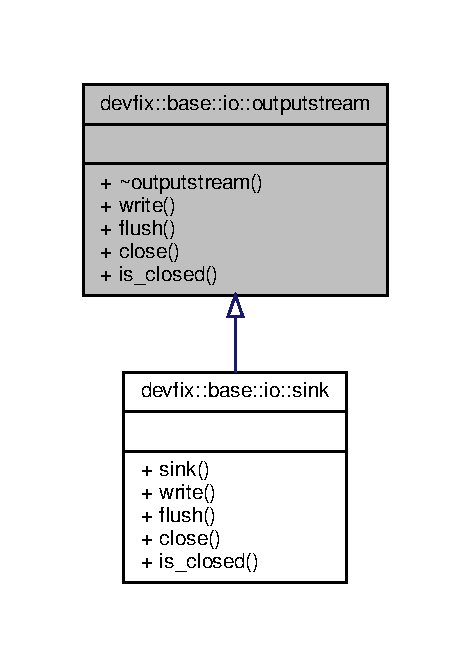
\includegraphics[width=226pt]{structdevfix_1_1base_1_1io_1_1outputstream__inherit__graph}
\end{center}
\end{figure}
\subsection*{Public Member Functions}
\begin{DoxyCompactItemize}
\item 
virtual \hyperlink{structdevfix_1_1base_1_1io_1_1outputstream_a9154a8859d44c7929c98fb83e03047e3}{$\sim$outputstream} ()=default
\item 
virtual void \hyperlink{structdevfix_1_1base_1_1io_1_1outputstream_ac7e5fcd6883c7c8f53356a4eb8284c00}{write} (const void $\ast$buf, std\+::size\+\_\+t len)=0
\begin{DoxyCompactList}\small\item\em Writes len bytes from the specified buffer to this output stream. \end{DoxyCompactList}\item 
virtual void \hyperlink{structdevfix_1_1base_1_1io_1_1outputstream_a3fe3b34675a2d70331e6ca235388e0cc}{flush} ()=0
\begin{DoxyCompactList}\small\item\em Flushes this {\itshape outputstream} and forces any buffered output bytes to be written out. \end{DoxyCompactList}\item 
virtual void \hyperlink{structdevfix_1_1base_1_1io_1_1outputstream_a060c2e7040e6bb831b8150f64bd8abf7}{close} ()=0
\begin{DoxyCompactList}\small\item\em Closes this {\itshape outputstream} and releases any system resources associated with this stream. \end{DoxyCompactList}\item 
virtual bool \hyperlink{structdevfix_1_1base_1_1io_1_1outputstream_a52bd2eac8f6fbc496eab5138a48d2f06}{is\+\_\+closed} ()=0
\begin{DoxyCompactList}\small\item\em Returns if the {\itshape outputstream} is closed or available for further calls of output operations. \end{DoxyCompactList}\end{DoxyCompactItemize}


\subsection{Detailed Description}
Superclass of all classes representing an output stream of bytes. 

An output stream accepts output bytes and sends them to some sink. Applications that need to define a subclass of Output\+Stream must always provide a method that writes one byte of output. 

\subsection{Constructor \& Destructor Documentation}
\mbox{\Hypertarget{structdevfix_1_1base_1_1io_1_1outputstream_a9154a8859d44c7929c98fb83e03047e3}\label{structdevfix_1_1base_1_1io_1_1outputstream_a9154a8859d44c7929c98fb83e03047e3}} 
\index{devfix\+::base\+::io\+::outputstream@{devfix\+::base\+::io\+::outputstream}!````~outputstream@{$\sim$outputstream}}
\index{````~outputstream@{$\sim$outputstream}!devfix\+::base\+::io\+::outputstream@{devfix\+::base\+::io\+::outputstream}}
\subsubsection{\texorpdfstring{$\sim$outputstream()}{~outputstream()}}
{\footnotesize\ttfamily virtual devfix\+::base\+::io\+::outputstream\+::$\sim$outputstream (\begin{DoxyParamCaption}{ }\end{DoxyParamCaption})\hspace{0.3cm}{\ttfamily [virtual]}, {\ttfamily [default]}}



\subsection{Member Function Documentation}
\mbox{\Hypertarget{structdevfix_1_1base_1_1io_1_1outputstream_a060c2e7040e6bb831b8150f64bd8abf7}\label{structdevfix_1_1base_1_1io_1_1outputstream_a060c2e7040e6bb831b8150f64bd8abf7}} 
\index{devfix\+::base\+::io\+::outputstream@{devfix\+::base\+::io\+::outputstream}!close@{close}}
\index{close@{close}!devfix\+::base\+::io\+::outputstream@{devfix\+::base\+::io\+::outputstream}}
\subsubsection{\texorpdfstring{close()}{close()}}
{\footnotesize\ttfamily virtual void devfix\+::base\+::io\+::outputstream\+::close (\begin{DoxyParamCaption}{ }\end{DoxyParamCaption})\hspace{0.3cm}{\ttfamily [pure virtual]}}



Closes this {\itshape outputstream} and releases any system resources associated with this stream. 

The general contract of close is that it closes the output stream. A closed stream cannot perform output operations and cannot be reopened. 

Implemented in \hyperlink{structdevfix_1_1base_1_1io_1_1sink_a2d110d27baa88f462540e7fd59fb8b3c}{devfix\+::base\+::io\+::sink}.

\mbox{\Hypertarget{structdevfix_1_1base_1_1io_1_1outputstream_a3fe3b34675a2d70331e6ca235388e0cc}\label{structdevfix_1_1base_1_1io_1_1outputstream_a3fe3b34675a2d70331e6ca235388e0cc}} 
\index{devfix\+::base\+::io\+::outputstream@{devfix\+::base\+::io\+::outputstream}!flush@{flush}}
\index{flush@{flush}!devfix\+::base\+::io\+::outputstream@{devfix\+::base\+::io\+::outputstream}}
\subsubsection{\texorpdfstring{flush()}{flush()}}
{\footnotesize\ttfamily virtual void devfix\+::base\+::io\+::outputstream\+::flush (\begin{DoxyParamCaption}{ }\end{DoxyParamCaption})\hspace{0.3cm}{\ttfamily [pure virtual]}}



Flushes this {\itshape outputstream} and forces any buffered output bytes to be written out. 

The general contract of flush is that calling it is an indication that, if any bytes previously written have been buffered by the implementation of the output stream, such bytes should immediately be written to their intended destination.

If the intended destination of this stream is an abstraction provided by the underlying operating system, for example a file, then flushing the stream guarantees only that bytes previously written to the stream are passed to the operating system for writing; it does not guarantee that they are actually written to a physical device such as a disk drive. 

Implemented in \hyperlink{structdevfix_1_1base_1_1io_1_1sink_abf208747c9be8295972fbc4696ddc557}{devfix\+::base\+::io\+::sink}.

\mbox{\Hypertarget{structdevfix_1_1base_1_1io_1_1outputstream_a52bd2eac8f6fbc496eab5138a48d2f06}\label{structdevfix_1_1base_1_1io_1_1outputstream_a52bd2eac8f6fbc496eab5138a48d2f06}} 
\index{devfix\+::base\+::io\+::outputstream@{devfix\+::base\+::io\+::outputstream}!is\+\_\+closed@{is\+\_\+closed}}
\index{is\+\_\+closed@{is\+\_\+closed}!devfix\+::base\+::io\+::outputstream@{devfix\+::base\+::io\+::outputstream}}
\subsubsection{\texorpdfstring{is\+\_\+closed()}{is\_closed()}}
{\footnotesize\ttfamily virtual bool devfix\+::base\+::io\+::outputstream\+::is\+\_\+closed (\begin{DoxyParamCaption}{ }\end{DoxyParamCaption})\hspace{0.3cm}{\ttfamily [pure virtual]}}



Returns if the {\itshape outputstream} is closed or available for further calls of output operations. 

\begin{DoxyReturn}{Returns}
true if the {\itshape outputstream} got previously closed. 
\end{DoxyReturn}


Implemented in \hyperlink{structdevfix_1_1base_1_1io_1_1sink_a1e5782219f9256d8ff09385fa6f3b156}{devfix\+::base\+::io\+::sink}.

\mbox{\Hypertarget{structdevfix_1_1base_1_1io_1_1outputstream_ac7e5fcd6883c7c8f53356a4eb8284c00}\label{structdevfix_1_1base_1_1io_1_1outputstream_ac7e5fcd6883c7c8f53356a4eb8284c00}} 
\index{devfix\+::base\+::io\+::outputstream@{devfix\+::base\+::io\+::outputstream}!write@{write}}
\index{write@{write}!devfix\+::base\+::io\+::outputstream@{devfix\+::base\+::io\+::outputstream}}
\subsubsection{\texorpdfstring{write()}{write()}}
{\footnotesize\ttfamily virtual void devfix\+::base\+::io\+::outputstream\+::write (\begin{DoxyParamCaption}\item[{const void $\ast$}]{buf,  }\item[{std\+::size\+\_\+t}]{len }\end{DoxyParamCaption})\hspace{0.3cm}{\ttfamily [pure virtual]}}



Writes len bytes from the specified buffer to this output stream. 

Element b\mbox{[}0\mbox{]} is the first byte written and b\mbox{[}len-\/1\mbox{]} is the last byte written by this operation.


\begin{DoxyParams}{Parameters}
{\em buf} & the data. \\
\hline
{\em len} & the number of bytes to write. \\
\hline
\end{DoxyParams}


Implemented in \hyperlink{structdevfix_1_1base_1_1io_1_1sink_a6eade9933d316139e952b7a442f3c56d}{devfix\+::base\+::io\+::sink}.



The documentation for this struct was generated from the following file\+:\begin{DoxyCompactItemize}
\item 
devfix/base/io/\hyperlink{outputstream_8h}{outputstream.\+h}\end{DoxyCompactItemize}

\hypertarget{structdevfix_1_1net_1_1serversocket}{}\section{devfix\+:\+:net\+:\+:serversocket Struct Reference}
\label{structdevfix_1_1net_1_1serversocket}\index{devfix\+::net\+::serversocket@{devfix\+::net\+::serversocket}}


{\ttfamily \#include $<$serversocket.\+h$>$}

\subsection*{Public Member Functions}
\begin{DoxyCompactItemize}
\item 
virtual \hyperlink{structdevfix_1_1net_1_1serversocket_afd9f315c4018808c790478710f52d8ab}{$\sim$serversocket} ()=default
\item 
virtual std\+::unique\+\_\+ptr$<$ \hyperlink{structdevfix_1_1net_1_1socket}{socket} $>$ \hyperlink{structdevfix_1_1net_1_1serversocket_a7b3ea6aad486060acdd1385a08f7db81}{accept} ()=0
\item 
virtual const \hyperlink{structdevfix_1_1net_1_1inetaddress}{inetaddress} \& \hyperlink{structdevfix_1_1net_1_1serversocket_a087a819b8173bfa101ea65ea8a17eb8c}{get\+\_\+address} () const noexcept=0
\item 
virtual bool \hyperlink{structdevfix_1_1net_1_1serversocket_a7efdb1f57d0e482542fda50a2403230d}{get\+\_\+reuse\+\_\+address} () const noexcept=0
\item 
virtual void \hyperlink{structdevfix_1_1net_1_1serversocket_ae67a25cf26fe54ce7b10d07ff9219ce7}{set\+\_\+accept\+\_\+timeout} (\hyperlink{structdevfix_1_1net_1_1socket_a80a3bf4cb7292bae31ea9c6575539c68}{socket\+::timeout\+\_\+t} timeout)=0
\item 
virtual \hyperlink{structdevfix_1_1net_1_1socket_a80a3bf4cb7292bae31ea9c6575539c68}{socket\+::timeout\+\_\+t} \hyperlink{structdevfix_1_1net_1_1serversocket_acde0979277bf9536f54bb0fb6a9cc881}{get\+\_\+accept\+\_\+timeout} () const noexcept=0
\item 
virtual void \hyperlink{structdevfix_1_1net_1_1serversocket_ab1762c3364c8298dbac6c3dd67a1e7aa}{close} ()=0
\item 
virtual bool \hyperlink{structdevfix_1_1net_1_1serversocket_a37cc4e3ecede2a0bc52f90e49fcbe4a9}{is\+\_\+closed} () const noexcept=0
\end{DoxyCompactItemize}


\subsection{Constructor \& Destructor Documentation}
\mbox{\Hypertarget{structdevfix_1_1net_1_1serversocket_afd9f315c4018808c790478710f52d8ab}\label{structdevfix_1_1net_1_1serversocket_afd9f315c4018808c790478710f52d8ab}} 
\index{devfix\+::net\+::serversocket@{devfix\+::net\+::serversocket}!````~serversocket@{$\sim$serversocket}}
\index{````~serversocket@{$\sim$serversocket}!devfix\+::net\+::serversocket@{devfix\+::net\+::serversocket}}
\subsubsection{\texorpdfstring{$\sim$serversocket()}{~serversocket()}}
{\footnotesize\ttfamily virtual devfix\+::net\+::serversocket\+::$\sim$serversocket (\begin{DoxyParamCaption}{ }\end{DoxyParamCaption})\hspace{0.3cm}{\ttfamily [virtual]}, {\ttfamily [default]}}



\subsection{Member Function Documentation}
\mbox{\Hypertarget{structdevfix_1_1net_1_1serversocket_a7b3ea6aad486060acdd1385a08f7db81}\label{structdevfix_1_1net_1_1serversocket_a7b3ea6aad486060acdd1385a08f7db81}} 
\index{devfix\+::net\+::serversocket@{devfix\+::net\+::serversocket}!accept@{accept}}
\index{accept@{accept}!devfix\+::net\+::serversocket@{devfix\+::net\+::serversocket}}
\subsubsection{\texorpdfstring{accept()}{accept()}}
{\footnotesize\ttfamily virtual std\+::unique\+\_\+ptr$<$\hyperlink{structdevfix_1_1net_1_1socket}{socket}$>$ devfix\+::net\+::serversocket\+::accept (\begin{DoxyParamCaption}{ }\end{DoxyParamCaption})\hspace{0.3cm}{\ttfamily [pure virtual]}}

\mbox{\Hypertarget{structdevfix_1_1net_1_1serversocket_ab1762c3364c8298dbac6c3dd67a1e7aa}\label{structdevfix_1_1net_1_1serversocket_ab1762c3364c8298dbac6c3dd67a1e7aa}} 
\index{devfix\+::net\+::serversocket@{devfix\+::net\+::serversocket}!close@{close}}
\index{close@{close}!devfix\+::net\+::serversocket@{devfix\+::net\+::serversocket}}
\subsubsection{\texorpdfstring{close()}{close()}}
{\footnotesize\ttfamily virtual void devfix\+::net\+::serversocket\+::close (\begin{DoxyParamCaption}{ }\end{DoxyParamCaption})\hspace{0.3cm}{\ttfamily [pure virtual]}}

\mbox{\Hypertarget{structdevfix_1_1net_1_1serversocket_acde0979277bf9536f54bb0fb6a9cc881}\label{structdevfix_1_1net_1_1serversocket_acde0979277bf9536f54bb0fb6a9cc881}} 
\index{devfix\+::net\+::serversocket@{devfix\+::net\+::serversocket}!get\+\_\+accept\+\_\+timeout@{get\+\_\+accept\+\_\+timeout}}
\index{get\+\_\+accept\+\_\+timeout@{get\+\_\+accept\+\_\+timeout}!devfix\+::net\+::serversocket@{devfix\+::net\+::serversocket}}
\subsubsection{\texorpdfstring{get\+\_\+accept\+\_\+timeout()}{get\_accept\_timeout()}}
{\footnotesize\ttfamily virtual \hyperlink{structdevfix_1_1net_1_1socket_a80a3bf4cb7292bae31ea9c6575539c68}{socket\+::timeout\+\_\+t} devfix\+::net\+::serversocket\+::get\+\_\+accept\+\_\+timeout (\begin{DoxyParamCaption}{ }\end{DoxyParamCaption}) const\hspace{0.3cm}{\ttfamily [pure virtual]}, {\ttfamily [noexcept]}}

\mbox{\Hypertarget{structdevfix_1_1net_1_1serversocket_a087a819b8173bfa101ea65ea8a17eb8c}\label{structdevfix_1_1net_1_1serversocket_a087a819b8173bfa101ea65ea8a17eb8c}} 
\index{devfix\+::net\+::serversocket@{devfix\+::net\+::serversocket}!get\+\_\+address@{get\+\_\+address}}
\index{get\+\_\+address@{get\+\_\+address}!devfix\+::net\+::serversocket@{devfix\+::net\+::serversocket}}
\subsubsection{\texorpdfstring{get\+\_\+address()}{get\_address()}}
{\footnotesize\ttfamily virtual const \hyperlink{structdevfix_1_1net_1_1inetaddress}{inetaddress}\& devfix\+::net\+::serversocket\+::get\+\_\+address (\begin{DoxyParamCaption}{ }\end{DoxyParamCaption}) const\hspace{0.3cm}{\ttfamily [pure virtual]}, {\ttfamily [noexcept]}}

\mbox{\Hypertarget{structdevfix_1_1net_1_1serversocket_a7efdb1f57d0e482542fda50a2403230d}\label{structdevfix_1_1net_1_1serversocket_a7efdb1f57d0e482542fda50a2403230d}} 
\index{devfix\+::net\+::serversocket@{devfix\+::net\+::serversocket}!get\+\_\+reuse\+\_\+address@{get\+\_\+reuse\+\_\+address}}
\index{get\+\_\+reuse\+\_\+address@{get\+\_\+reuse\+\_\+address}!devfix\+::net\+::serversocket@{devfix\+::net\+::serversocket}}
\subsubsection{\texorpdfstring{get\+\_\+reuse\+\_\+address()}{get\_reuse\_address()}}
{\footnotesize\ttfamily virtual bool devfix\+::net\+::serversocket\+::get\+\_\+reuse\+\_\+address (\begin{DoxyParamCaption}{ }\end{DoxyParamCaption}) const\hspace{0.3cm}{\ttfamily [pure virtual]}, {\ttfamily [noexcept]}}

\mbox{\Hypertarget{structdevfix_1_1net_1_1serversocket_a37cc4e3ecede2a0bc52f90e49fcbe4a9}\label{structdevfix_1_1net_1_1serversocket_a37cc4e3ecede2a0bc52f90e49fcbe4a9}} 
\index{devfix\+::net\+::serversocket@{devfix\+::net\+::serversocket}!is\+\_\+closed@{is\+\_\+closed}}
\index{is\+\_\+closed@{is\+\_\+closed}!devfix\+::net\+::serversocket@{devfix\+::net\+::serversocket}}
\subsubsection{\texorpdfstring{is\+\_\+closed()}{is\_closed()}}
{\footnotesize\ttfamily virtual bool devfix\+::net\+::serversocket\+::is\+\_\+closed (\begin{DoxyParamCaption}{ }\end{DoxyParamCaption}) const\hspace{0.3cm}{\ttfamily [pure virtual]}, {\ttfamily [noexcept]}}

\mbox{\Hypertarget{structdevfix_1_1net_1_1serversocket_ae67a25cf26fe54ce7b10d07ff9219ce7}\label{structdevfix_1_1net_1_1serversocket_ae67a25cf26fe54ce7b10d07ff9219ce7}} 
\index{devfix\+::net\+::serversocket@{devfix\+::net\+::serversocket}!set\+\_\+accept\+\_\+timeout@{set\+\_\+accept\+\_\+timeout}}
\index{set\+\_\+accept\+\_\+timeout@{set\+\_\+accept\+\_\+timeout}!devfix\+::net\+::serversocket@{devfix\+::net\+::serversocket}}
\subsubsection{\texorpdfstring{set\+\_\+accept\+\_\+timeout()}{set\_accept\_timeout()}}
{\footnotesize\ttfamily virtual void devfix\+::net\+::serversocket\+::set\+\_\+accept\+\_\+timeout (\begin{DoxyParamCaption}\item[{\hyperlink{structdevfix_1_1net_1_1socket_a80a3bf4cb7292bae31ea9c6575539c68}{socket\+::timeout\+\_\+t}}]{timeout }\end{DoxyParamCaption})\hspace{0.3cm}{\ttfamily [pure virtual]}}



The documentation for this struct was generated from the following file\+:\begin{DoxyCompactItemize}
\item 
devfix/net/\hyperlink{serversocket_8h}{serversocket.\+h}\end{DoxyCompactItemize}

\hypertarget{structdevfix_1_1base_1_1io_1_1sink}{}\section{devfix\+:\+:base\+:\+:io\+:\+:sink Struct Reference}
\label{structdevfix_1_1base_1_1io_1_1sink}\index{devfix\+::base\+::io\+::sink@{devfix\+::base\+::io\+::sink}}


Inheritance diagram for devfix\+:\+:base\+:\+:io\+:\+:sink\+:
% FIG 0


Collaboration diagram for devfix\+:\+:base\+:\+:io\+:\+:sink\+:
% FIG 1
\subsection*{Public Member Functions}
\begin{DoxyCompactItemize}
\item 
\mbox{\Hypertarget{structdevfix_1_1base_1_1io_1_1sink_a5e065482904521fde4ac8d0e378529c8}\label{structdevfix_1_1base_1_1io_1_1sink_a5e065482904521fde4ac8d0e378529c8}} 
{\bfseries sink} (write\+\_\+t write, flush\+\_\+t flush, close\+\_\+t close=D\+E\+F\+A\+U\+L\+T\+\_\+\+C\+L\+O\+SE, is\+\_\+closed\+\_\+t is\+\_\+closed=D\+E\+F\+A\+U\+L\+T\+\_\+\+I\+S\+\_\+\+C\+L\+O\+S\+ED)
\item 
\mbox{\Hypertarget{structdevfix_1_1base_1_1io_1_1sink_a912eebd869f230d506a2c8fcd69051b4}\label{structdevfix_1_1base_1_1io_1_1sink_a912eebd869f230d506a2c8fcd69051b4}} 
void {\bfseries write} (void $\ast$buf, std\+::size\+\_\+t len)
\item 
\mbox{\Hypertarget{structdevfix_1_1base_1_1io_1_1sink_abf208747c9be8295972fbc4696ddc557}\label{structdevfix_1_1base_1_1io_1_1sink_abf208747c9be8295972fbc4696ddc557}} 
void {\bfseries flush} ()
\item 
\mbox{\Hypertarget{structdevfix_1_1base_1_1io_1_1sink_a2d110d27baa88f462540e7fd59fb8b3c}\label{structdevfix_1_1base_1_1io_1_1sink_a2d110d27baa88f462540e7fd59fb8b3c}} 
void {\bfseries close} ()
\item 
\mbox{\Hypertarget{structdevfix_1_1base_1_1io_1_1sink_a1e5782219f9256d8ff09385fa6f3b156}\label{structdevfix_1_1base_1_1io_1_1sink_a1e5782219f9256d8ff09385fa6f3b156}} 
bool {\bfseries is\+\_\+closed} ()
\end{DoxyCompactItemize}


The documentation for this struct was generated from the following files\+:\begin{DoxyCompactItemize}
\item 
devfix/base/io/sink.\+h\item 
devfix/base/io/sink.\+cpp\end{DoxyCompactItemize}

\hypertarget{structdevfix_1_1net_1_1socket}{}\section{devfix\+:\+:net\+:\+:socket Struct Reference}
\label{structdevfix_1_1net_1_1socket}\index{devfix\+::net\+::socket@{devfix\+::net\+::socket}}


{\ttfamily \#include $<$socket.\+h$>$}

\subsection*{Public Types}
\begin{DoxyCompactItemize}
\item 
typedef std\+::uint32\+\_\+t \hyperlink{structdevfix_1_1net_1_1socket_a80a3bf4cb7292bae31ea9c6575539c68}{timeout\+\_\+t}
\end{DoxyCompactItemize}
\subsection*{Public Member Functions}
\begin{DoxyCompactItemize}
\item 
virtual \hyperlink{structdevfix_1_1net_1_1socket_ad9d4d9643894e213faefd4e37938f1fe}{$\sim$socket} ()=default
\item 
virtual const \hyperlink{structdevfix_1_1net_1_1inetaddress}{inetaddress} \& \hyperlink{structdevfix_1_1net_1_1socket_a570b728ca81a3d47ca7733ff21063318}{get\+\_\+local\+\_\+address} () const noexcept=0
\item 
virtual const \hyperlink{structdevfix_1_1net_1_1inetaddress}{inetaddress} \& \hyperlink{structdevfix_1_1net_1_1socket_afb69dcc8da66eb15a927d031f50a4ba2}{get\+\_\+remote\+\_\+address} () const noexcept=0
\item 
virtual \hyperlink{structdevfix_1_1base_1_1io_1_1inputstream}{base\+::io\+::inputstream} \& \hyperlink{structdevfix_1_1net_1_1socket_a3a00115497ccb83e8497a7e33be06b03}{get\+\_\+inputstream} () const noexcept=0
\item 
virtual \hyperlink{structdevfix_1_1base_1_1io_1_1outputstream}{base\+::io\+::outputstream} \& \hyperlink{structdevfix_1_1net_1_1socket_ac0320fa786f14778a3a1e2796d9dce57}{get\+\_\+outputstream} () const noexcept=0
\item 
virtual void \hyperlink{structdevfix_1_1net_1_1socket_a3fa8d7dcd44e7740b29ad6674005eb5d}{set\+\_\+interrupted} (bool \hyperlink{structdevfix_1_1net_1_1socket_a7cfe151f1124d46fb19fad0c374c9352}{interrupted}) noexcept=0
\item 
virtual bool \hyperlink{structdevfix_1_1net_1_1socket_a7cfe151f1124d46fb19fad0c374c9352}{interrupted} () const noexcept=0
\item 
virtual void \hyperlink{structdevfix_1_1net_1_1socket_ae1cf3b2c4f5d39225d6585c387f967d5}{set\+\_\+timeout} (\hyperlink{structdevfix_1_1net_1_1socket_a80a3bf4cb7292bae31ea9c6575539c68}{timeout\+\_\+t} timeout) noexcept=0
\item 
virtual \hyperlink{structdevfix_1_1net_1_1socket_a80a3bf4cb7292bae31ea9c6575539c68}{timeout\+\_\+t} \hyperlink{structdevfix_1_1net_1_1socket_afac86b6ad30a758ce590e7a144764967}{get\+\_\+timeout} () const noexcept=0
\end{DoxyCompactItemize}
\subsection*{Static Public Attributes}
\begin{DoxyCompactItemize}
\item 
static constexpr \hyperlink{structdevfix_1_1net_1_1socket_a80a3bf4cb7292bae31ea9c6575539c68}{timeout\+\_\+t} \hyperlink{structdevfix_1_1net_1_1socket_a1bd6468be497aed208ad6d5632683a5d}{D\+E\+F\+A\+U\+L\+T\+\_\+\+T\+I\+M\+E\+O\+UT} = 3000
\begin{DoxyCompactList}\small\item\em default read timeout in milliseconds \end{DoxyCompactList}\item 
static constexpr \hyperlink{structdevfix_1_1net_1_1socket_a80a3bf4cb7292bae31ea9c6575539c68}{timeout\+\_\+t} \hyperlink{structdevfix_1_1net_1_1socket_a77c3214eb436d06825a4cc2aafcc63ce}{D\+E\+F\+A\+U\+L\+T\+\_\+\+R\+E\+A\+D\+\_\+\+B\+L\+O\+C\+K\+I\+N\+G\+\_\+\+T\+I\+ME} = 100
\begin{DoxyCompactList}\small\item\em default read timeout until refresh in milliseconds \end{DoxyCompactList}\end{DoxyCompactItemize}


\subsection{Member Typedef Documentation}
\mbox{\Hypertarget{structdevfix_1_1net_1_1socket_a80a3bf4cb7292bae31ea9c6575539c68}\label{structdevfix_1_1net_1_1socket_a80a3bf4cb7292bae31ea9c6575539c68}} 
\index{devfix\+::net\+::socket@{devfix\+::net\+::socket}!timeout\+\_\+t@{timeout\+\_\+t}}
\index{timeout\+\_\+t@{timeout\+\_\+t}!devfix\+::net\+::socket@{devfix\+::net\+::socket}}
\subsubsection{\texorpdfstring{timeout\+\_\+t}{timeout\_t}}
{\footnotesize\ttfamily typedef std\+::uint32\+\_\+t \hyperlink{structdevfix_1_1net_1_1socket_a80a3bf4cb7292bae31ea9c6575539c68}{devfix\+::net\+::socket\+::timeout\+\_\+t}}



\subsection{Constructor \& Destructor Documentation}
\mbox{\Hypertarget{structdevfix_1_1net_1_1socket_ad9d4d9643894e213faefd4e37938f1fe}\label{structdevfix_1_1net_1_1socket_ad9d4d9643894e213faefd4e37938f1fe}} 
\index{devfix\+::net\+::socket@{devfix\+::net\+::socket}!````~socket@{$\sim$socket}}
\index{````~socket@{$\sim$socket}!devfix\+::net\+::socket@{devfix\+::net\+::socket}}
\subsubsection{\texorpdfstring{$\sim$socket()}{~socket()}}
{\footnotesize\ttfamily virtual devfix\+::net\+::socket\+::$\sim$socket (\begin{DoxyParamCaption}{ }\end{DoxyParamCaption})\hspace{0.3cm}{\ttfamily [virtual]}, {\ttfamily [default]}}



\subsection{Member Function Documentation}
\mbox{\Hypertarget{structdevfix_1_1net_1_1socket_a3a00115497ccb83e8497a7e33be06b03}\label{structdevfix_1_1net_1_1socket_a3a00115497ccb83e8497a7e33be06b03}} 
\index{devfix\+::net\+::socket@{devfix\+::net\+::socket}!get\+\_\+inputstream@{get\+\_\+inputstream}}
\index{get\+\_\+inputstream@{get\+\_\+inputstream}!devfix\+::net\+::socket@{devfix\+::net\+::socket}}
\subsubsection{\texorpdfstring{get\+\_\+inputstream()}{get\_inputstream()}}
{\footnotesize\ttfamily virtual \hyperlink{structdevfix_1_1base_1_1io_1_1inputstream}{base\+::io\+::inputstream}\& devfix\+::net\+::socket\+::get\+\_\+inputstream (\begin{DoxyParamCaption}{ }\end{DoxyParamCaption}) const\hspace{0.3cm}{\ttfamily [pure virtual]}, {\ttfamily [noexcept]}}

\mbox{\Hypertarget{structdevfix_1_1net_1_1socket_a570b728ca81a3d47ca7733ff21063318}\label{structdevfix_1_1net_1_1socket_a570b728ca81a3d47ca7733ff21063318}} 
\index{devfix\+::net\+::socket@{devfix\+::net\+::socket}!get\+\_\+local\+\_\+address@{get\+\_\+local\+\_\+address}}
\index{get\+\_\+local\+\_\+address@{get\+\_\+local\+\_\+address}!devfix\+::net\+::socket@{devfix\+::net\+::socket}}
\subsubsection{\texorpdfstring{get\+\_\+local\+\_\+address()}{get\_local\_address()}}
{\footnotesize\ttfamily virtual const \hyperlink{structdevfix_1_1net_1_1inetaddress}{inetaddress}\& devfix\+::net\+::socket\+::get\+\_\+local\+\_\+address (\begin{DoxyParamCaption}{ }\end{DoxyParamCaption}) const\hspace{0.3cm}{\ttfamily [pure virtual]}, {\ttfamily [noexcept]}}

\mbox{\Hypertarget{structdevfix_1_1net_1_1socket_ac0320fa786f14778a3a1e2796d9dce57}\label{structdevfix_1_1net_1_1socket_ac0320fa786f14778a3a1e2796d9dce57}} 
\index{devfix\+::net\+::socket@{devfix\+::net\+::socket}!get\+\_\+outputstream@{get\+\_\+outputstream}}
\index{get\+\_\+outputstream@{get\+\_\+outputstream}!devfix\+::net\+::socket@{devfix\+::net\+::socket}}
\subsubsection{\texorpdfstring{get\+\_\+outputstream()}{get\_outputstream()}}
{\footnotesize\ttfamily virtual \hyperlink{structdevfix_1_1base_1_1io_1_1outputstream}{base\+::io\+::outputstream}\& devfix\+::net\+::socket\+::get\+\_\+outputstream (\begin{DoxyParamCaption}{ }\end{DoxyParamCaption}) const\hspace{0.3cm}{\ttfamily [pure virtual]}, {\ttfamily [noexcept]}}

\mbox{\Hypertarget{structdevfix_1_1net_1_1socket_afb69dcc8da66eb15a927d031f50a4ba2}\label{structdevfix_1_1net_1_1socket_afb69dcc8da66eb15a927d031f50a4ba2}} 
\index{devfix\+::net\+::socket@{devfix\+::net\+::socket}!get\+\_\+remote\+\_\+address@{get\+\_\+remote\+\_\+address}}
\index{get\+\_\+remote\+\_\+address@{get\+\_\+remote\+\_\+address}!devfix\+::net\+::socket@{devfix\+::net\+::socket}}
\subsubsection{\texorpdfstring{get\+\_\+remote\+\_\+address()}{get\_remote\_address()}}
{\footnotesize\ttfamily virtual const \hyperlink{structdevfix_1_1net_1_1inetaddress}{inetaddress}\& devfix\+::net\+::socket\+::get\+\_\+remote\+\_\+address (\begin{DoxyParamCaption}{ }\end{DoxyParamCaption}) const\hspace{0.3cm}{\ttfamily [pure virtual]}, {\ttfamily [noexcept]}}

\mbox{\Hypertarget{structdevfix_1_1net_1_1socket_afac86b6ad30a758ce590e7a144764967}\label{structdevfix_1_1net_1_1socket_afac86b6ad30a758ce590e7a144764967}} 
\index{devfix\+::net\+::socket@{devfix\+::net\+::socket}!get\+\_\+timeout@{get\+\_\+timeout}}
\index{get\+\_\+timeout@{get\+\_\+timeout}!devfix\+::net\+::socket@{devfix\+::net\+::socket}}
\subsubsection{\texorpdfstring{get\+\_\+timeout()}{get\_timeout()}}
{\footnotesize\ttfamily virtual \hyperlink{structdevfix_1_1net_1_1socket_a80a3bf4cb7292bae31ea9c6575539c68}{timeout\+\_\+t} devfix\+::net\+::socket\+::get\+\_\+timeout (\begin{DoxyParamCaption}{ }\end{DoxyParamCaption}) const\hspace{0.3cm}{\ttfamily [pure virtual]}, {\ttfamily [noexcept]}}

\mbox{\Hypertarget{structdevfix_1_1net_1_1socket_a7cfe151f1124d46fb19fad0c374c9352}\label{structdevfix_1_1net_1_1socket_a7cfe151f1124d46fb19fad0c374c9352}} 
\index{devfix\+::net\+::socket@{devfix\+::net\+::socket}!interrupted@{interrupted}}
\index{interrupted@{interrupted}!devfix\+::net\+::socket@{devfix\+::net\+::socket}}
\subsubsection{\texorpdfstring{interrupted()}{interrupted()}}
{\footnotesize\ttfamily virtual bool devfix\+::net\+::socket\+::interrupted (\begin{DoxyParamCaption}{ }\end{DoxyParamCaption}) const\hspace{0.3cm}{\ttfamily [pure virtual]}, {\ttfamily [noexcept]}}

\begin{DoxyReturn}{Returns}
true if the socket is interrupted. 
\end{DoxyReturn}
\mbox{\Hypertarget{structdevfix_1_1net_1_1socket_a3fa8d7dcd44e7740b29ad6674005eb5d}\label{structdevfix_1_1net_1_1socket_a3fa8d7dcd44e7740b29ad6674005eb5d}} 
\index{devfix\+::net\+::socket@{devfix\+::net\+::socket}!set\+\_\+interrupted@{set\+\_\+interrupted}}
\index{set\+\_\+interrupted@{set\+\_\+interrupted}!devfix\+::net\+::socket@{devfix\+::net\+::socket}}
\subsubsection{\texorpdfstring{set\+\_\+interrupted()}{set\_interrupted()}}
{\footnotesize\ttfamily virtual void devfix\+::net\+::socket\+::set\+\_\+interrupted (\begin{DoxyParamCaption}\item[{bool}]{interrupted }\end{DoxyParamCaption})\hspace{0.3cm}{\ttfamily [pure virtual]}, {\ttfamily [noexcept]}}

Set the socket as interrupted. 
\begin{DoxyParams}{Parameters}
{\em interrupted} & If set true, any read call returns after the read blocking time expired and throws an error. \\
\hline
\end{DoxyParams}
\mbox{\Hypertarget{structdevfix_1_1net_1_1socket_ae1cf3b2c4f5d39225d6585c387f967d5}\label{structdevfix_1_1net_1_1socket_ae1cf3b2c4f5d39225d6585c387f967d5}} 
\index{devfix\+::net\+::socket@{devfix\+::net\+::socket}!set\+\_\+timeout@{set\+\_\+timeout}}
\index{set\+\_\+timeout@{set\+\_\+timeout}!devfix\+::net\+::socket@{devfix\+::net\+::socket}}
\subsubsection{\texorpdfstring{set\+\_\+timeout()}{set\_timeout()}}
{\footnotesize\ttfamily virtual void devfix\+::net\+::socket\+::set\+\_\+timeout (\begin{DoxyParamCaption}\item[{\hyperlink{structdevfix_1_1net_1_1socket_a80a3bf4cb7292bae31ea9c6575539c68}{timeout\+\_\+t}}]{timeout }\end{DoxyParamCaption})\hspace{0.3cm}{\ttfamily [pure virtual]}, {\ttfamily [noexcept]}}



\subsection{Member Data Documentation}
\mbox{\Hypertarget{structdevfix_1_1net_1_1socket_a77c3214eb436d06825a4cc2aafcc63ce}\label{structdevfix_1_1net_1_1socket_a77c3214eb436d06825a4cc2aafcc63ce}} 
\index{devfix\+::net\+::socket@{devfix\+::net\+::socket}!D\+E\+F\+A\+U\+L\+T\+\_\+\+R\+E\+A\+D\+\_\+\+B\+L\+O\+C\+K\+I\+N\+G\+\_\+\+T\+I\+ME@{D\+E\+F\+A\+U\+L\+T\+\_\+\+R\+E\+A\+D\+\_\+\+B\+L\+O\+C\+K\+I\+N\+G\+\_\+\+T\+I\+ME}}
\index{D\+E\+F\+A\+U\+L\+T\+\_\+\+R\+E\+A\+D\+\_\+\+B\+L\+O\+C\+K\+I\+N\+G\+\_\+\+T\+I\+ME@{D\+E\+F\+A\+U\+L\+T\+\_\+\+R\+E\+A\+D\+\_\+\+B\+L\+O\+C\+K\+I\+N\+G\+\_\+\+T\+I\+ME}!devfix\+::net\+::socket@{devfix\+::net\+::socket}}
\subsubsection{\texorpdfstring{D\+E\+F\+A\+U\+L\+T\+\_\+\+R\+E\+A\+D\+\_\+\+B\+L\+O\+C\+K\+I\+N\+G\+\_\+\+T\+I\+ME}{DEFAULT\_READ\_BLOCKING\_TIME}}
{\footnotesize\ttfamily constexpr \hyperlink{structdevfix_1_1net_1_1socket_a80a3bf4cb7292bae31ea9c6575539c68}{timeout\+\_\+t} devfix\+::net\+::socket\+::\+D\+E\+F\+A\+U\+L\+T\+\_\+\+R\+E\+A\+D\+\_\+\+B\+L\+O\+C\+K\+I\+N\+G\+\_\+\+T\+I\+ME = 100\hspace{0.3cm}{\ttfamily [static]}}



default read timeout until refresh in milliseconds 

\mbox{\Hypertarget{structdevfix_1_1net_1_1socket_a1bd6468be497aed208ad6d5632683a5d}\label{structdevfix_1_1net_1_1socket_a1bd6468be497aed208ad6d5632683a5d}} 
\index{devfix\+::net\+::socket@{devfix\+::net\+::socket}!D\+E\+F\+A\+U\+L\+T\+\_\+\+T\+I\+M\+E\+O\+UT@{D\+E\+F\+A\+U\+L\+T\+\_\+\+T\+I\+M\+E\+O\+UT}}
\index{D\+E\+F\+A\+U\+L\+T\+\_\+\+T\+I\+M\+E\+O\+UT@{D\+E\+F\+A\+U\+L\+T\+\_\+\+T\+I\+M\+E\+O\+UT}!devfix\+::net\+::socket@{devfix\+::net\+::socket}}
\subsubsection{\texorpdfstring{D\+E\+F\+A\+U\+L\+T\+\_\+\+T\+I\+M\+E\+O\+UT}{DEFAULT\_TIMEOUT}}
{\footnotesize\ttfamily constexpr \hyperlink{structdevfix_1_1net_1_1socket_a80a3bf4cb7292bae31ea9c6575539c68}{timeout\+\_\+t} devfix\+::net\+::socket\+::\+D\+E\+F\+A\+U\+L\+T\+\_\+\+T\+I\+M\+E\+O\+UT = 3000\hspace{0.3cm}{\ttfamily [static]}}



default read timeout in milliseconds 



The documentation for this struct was generated from the following file\+:\begin{DoxyCompactItemize}
\item 
devfix/net/\hyperlink{socket_8h}{socket.\+h}\end{DoxyCompactItemize}

\hypertarget{structdevfix_1_1net_1_1socketexception}{}\section{devfix\+:\+:net\+:\+:socketexception Struct Reference}
\label{structdevfix_1_1net_1_1socketexception}\index{devfix\+::net\+::socketexception@{devfix\+::net\+::socketexception}}


Thrown to indicate that there is an error creating or accessing a Socket.  




{\ttfamily \#include $<$socketexception.\+h$>$}



Inheritance diagram for devfix\+:\+:net\+:\+:socketexception\+:
\nopagebreak
\begin{figure}[H]
\begin{center}
\leavevmode
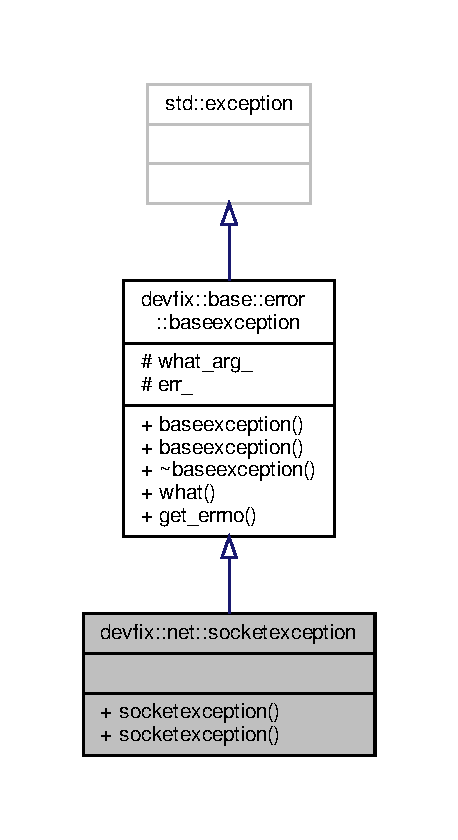
\includegraphics[width=220pt]{structdevfix_1_1net_1_1socketexception__inherit__graph}
\end{center}
\end{figure}
\subsection*{Public Member Functions}
\begin{DoxyCompactItemize}
\item 
\hyperlink{structdevfix_1_1net_1_1socketexception_aeab5d004d494103b37156a5f23a5296a}{socketexception} (const std\+::string \&what\+\_\+arg, int err=-\/1)
\item 
\hyperlink{structdevfix_1_1net_1_1socketexception_a6da69f635eb11f932a0e960545d023bd}{socketexception} (const char $\ast$what\+\_\+arg, int err=-\/1)
\end{DoxyCompactItemize}
\subsection*{Additional Inherited Members}


\subsection{Detailed Description}
Thrown to indicate that there is an error creating or accessing a Socket. 

\subsection{Constructor \& Destructor Documentation}
\mbox{\Hypertarget{structdevfix_1_1net_1_1socketexception_aeab5d004d494103b37156a5f23a5296a}\label{structdevfix_1_1net_1_1socketexception_aeab5d004d494103b37156a5f23a5296a}} 
\index{devfix\+::net\+::socketexception@{devfix\+::net\+::socketexception}!socketexception@{socketexception}}
\index{socketexception@{socketexception}!devfix\+::net\+::socketexception@{devfix\+::net\+::socketexception}}
\subsubsection{\texorpdfstring{socketexception()}{socketexception()}\hspace{0.1cm}{\footnotesize\ttfamily [1/2]}}
{\footnotesize\ttfamily devfix\+::net\+::socketexception\+::socketexception (\begin{DoxyParamCaption}\item[{const std\+::string \&}]{what\+\_\+arg,  }\item[{int}]{err = {\ttfamily -\/1} }\end{DoxyParamCaption})\hspace{0.3cm}{\ttfamily [inline]}, {\ttfamily [explicit]}}

Constructs the error object with what\+\_\+arg as explanatory string that can be accessed through \hyperlink{structdevfix_1_1base_1_1error_1_1baseexception_a16327152a55d65b1e537825231fbd452}{what()}. 
\begin{DoxyParams}{Parameters}
{\em what\+\_\+arg} & explanatory std\+::string \\
\hline
{\em err} & c error code (errno) \\
\hline
\end{DoxyParams}
\mbox{\Hypertarget{structdevfix_1_1net_1_1socketexception_a6da69f635eb11f932a0e960545d023bd}\label{structdevfix_1_1net_1_1socketexception_a6da69f635eb11f932a0e960545d023bd}} 
\index{devfix\+::net\+::socketexception@{devfix\+::net\+::socketexception}!socketexception@{socketexception}}
\index{socketexception@{socketexception}!devfix\+::net\+::socketexception@{devfix\+::net\+::socketexception}}
\subsubsection{\texorpdfstring{socketexception()}{socketexception()}\hspace{0.1cm}{\footnotesize\ttfamily [2/2]}}
{\footnotesize\ttfamily devfix\+::net\+::socketexception\+::socketexception (\begin{DoxyParamCaption}\item[{const char $\ast$}]{what\+\_\+arg,  }\item[{int}]{err = {\ttfamily -\/1} }\end{DoxyParamCaption})\hspace{0.3cm}{\ttfamily [inline]}, {\ttfamily [explicit]}}

Constructs the error object with what\+\_\+arg as explanatory string that can be accessed through \hyperlink{structdevfix_1_1base_1_1error_1_1baseexception_a16327152a55d65b1e537825231fbd452}{what()}. 
\begin{DoxyParams}{Parameters}
{\em what\+\_\+arg} & explanatory c-\/string \\
\hline
{\em err} & c error code (errno) \\
\hline
\end{DoxyParams}


The documentation for this struct was generated from the following file\+:\begin{DoxyCompactItemize}
\item 
devfix/net/\hyperlink{socketexception_8h}{socketexception.\+h}\end{DoxyCompactItemize}

\hypertarget{structdevfix_1_1base_1_1io_1_1source}{}\section{devfix\+:\+:base\+:\+:io\+:\+:source Struct Reference}
\label{structdevfix_1_1base_1_1io_1_1source}\index{devfix\+::base\+::io\+::source@{devfix\+::base\+::io\+::source}}


Inheritance diagram for devfix\+:\+:base\+:\+:io\+:\+:source\+:
% FIG 0


Collaboration diagram for devfix\+:\+:base\+:\+:io\+:\+:source\+:
% FIG 1
\subsection*{Public Member Functions}
\begin{DoxyCompactItemize}
\item 
\mbox{\Hypertarget{structdevfix_1_1base_1_1io_1_1source_af8bef20f5b54153c3fd1fbc7daa263c5}\label{structdevfix_1_1base_1_1io_1_1source_af8bef20f5b54153c3fd1fbc7daa263c5}} 
{\bfseries source} (read\+\_\+t \hyperlink{structdevfix_1_1base_1_1io_1_1source_a9fbd4d20aa150910ced44018e1b3156a}{read}, skip\+\_\+t \hyperlink{structdevfix_1_1base_1_1io_1_1source_a21cb579307589cbc6f9e02d64c66f4b2}{skip}, available\+\_\+t \hyperlink{structdevfix_1_1base_1_1io_1_1source_a911f4ba79499a623de30cf16d3d26d47}{available}, close\+\_\+t \hyperlink{structdevfix_1_1base_1_1io_1_1source_aa00a381c8a166cbbc5dbf6de4b56590e}{close}=D\+E\+F\+A\+U\+L\+T\+\_\+\+C\+L\+O\+SE, is\+\_\+closed\+\_\+t \hyperlink{structdevfix_1_1base_1_1io_1_1source_a406834cf6651d48949b96d0ef49cc6c1}{is\+\_\+closed}=D\+E\+F\+A\+U\+L\+T\+\_\+\+I\+S\+\_\+\+C\+L\+O\+S\+ED)
\item 
void \hyperlink{structdevfix_1_1base_1_1io_1_1source_a9fbd4d20aa150910ced44018e1b3156a}{read} (void $\ast$buf, std\+::size\+\_\+t len) override
\begin{DoxyCompactList}\small\item\em Reads bytes from the input stream and stores them into the buffer. \end{DoxyCompactList}\item 
void \hyperlink{structdevfix_1_1base_1_1io_1_1source_a21cb579307589cbc6f9e02d64c66f4b2}{skip} (std\+::size\+\_\+t n) override
\begin{DoxyCompactList}\small\item\em Skips over and discards n bytes of data from this input stream. \end{DoxyCompactList}\item 
std\+::size\+\_\+t \hyperlink{structdevfix_1_1base_1_1io_1_1source_a911f4ba79499a623de30cf16d3d26d47}{available} () override
\begin{DoxyCompactList}\small\item\em Returns an estimate of the number of bytes that can be read (or skipped over) from this input stream without blocking by the next invocation of a method for this input stream. \end{DoxyCompactList}\item 
void \hyperlink{structdevfix_1_1base_1_1io_1_1source_aa00a381c8a166cbbc5dbf6de4b56590e}{close} () override
\begin{DoxyCompactList}\small\item\em Closes this input stream and releases any system resources associated with the stream. \end{DoxyCompactList}\item 
bool \hyperlink{structdevfix_1_1base_1_1io_1_1source_a406834cf6651d48949b96d0ef49cc6c1}{is\+\_\+closed} () override
\begin{DoxyCompactList}\small\item\em Returns if the {\itshape inputstream} is closed or available for further calls of input operations. \end{DoxyCompactList}\end{DoxyCompactItemize}


\subsection{Member Function Documentation}
\mbox{\Hypertarget{structdevfix_1_1base_1_1io_1_1source_a911f4ba79499a623de30cf16d3d26d47}\label{structdevfix_1_1base_1_1io_1_1source_a911f4ba79499a623de30cf16d3d26d47}} 
\index{devfix\+::base\+::io\+::source@{devfix\+::base\+::io\+::source}!available@{available}}
\index{available@{available}!devfix\+::base\+::io\+::source@{devfix\+::base\+::io\+::source}}
\subsubsection{\texorpdfstring{available()}{available()}}
{\footnotesize\ttfamily std\+::size\+\_\+t devfix\+::base\+::io\+::source\+::available (\begin{DoxyParamCaption}{ }\end{DoxyParamCaption})\hspace{0.3cm}{\ttfamily [override]}, {\ttfamily [virtual]}}



Returns an estimate of the number of bytes that can be read (or skipped over) from this input stream without blocking by the next invocation of a method for this input stream. 

A single read or skip of this many bytes will not block, but may read or skip fewer bytes.

Note that while some implementations of {\itshape inputstream} will return the total number of bytes in the stream, many will not. It is never correct to use the return value of this method to allocate a buffer intended to hold all data in this stream.

A subclass\textquotesingle{} implementation of this method may choose to throw an I\+O\+Exception if this input stream has been closed by invoking the \hyperlink{structdevfix_1_1base_1_1io_1_1source_aa00a381c8a166cbbc5dbf6de4b56590e}{close()} method.

This method should be overridden by subclasses.

\begin{DoxyReturn}{Returns}
an estimate of the number of bytes that can be read (or skipped over) from this input stream without blocking or 0 when it reaches the end of the input stream. 
\end{DoxyReturn}


Implements \hyperlink{structdevfix_1_1base_1_1io_1_1inputstream_ace04813af676b6c81fa452eb4d81a796}{devfix\+::base\+::io\+::inputstream}.

\mbox{\Hypertarget{structdevfix_1_1base_1_1io_1_1source_aa00a381c8a166cbbc5dbf6de4b56590e}\label{structdevfix_1_1base_1_1io_1_1source_aa00a381c8a166cbbc5dbf6de4b56590e}} 
\index{devfix\+::base\+::io\+::source@{devfix\+::base\+::io\+::source}!close@{close}}
\index{close@{close}!devfix\+::base\+::io\+::source@{devfix\+::base\+::io\+::source}}
\subsubsection{\texorpdfstring{close()}{close()}}
{\footnotesize\ttfamily void devfix\+::base\+::io\+::source\+::close (\begin{DoxyParamCaption}{ }\end{DoxyParamCaption})\hspace{0.3cm}{\ttfamily [override]}, {\ttfamily [virtual]}}



Closes this input stream and releases any system resources associated with the stream. 

A closed stream cannot perform input operations and cannot be reopened. 

Implements \hyperlink{structdevfix_1_1base_1_1io_1_1inputstream_a1188eff97757eb9625be91dfeca17af7}{devfix\+::base\+::io\+::inputstream}.

\mbox{\Hypertarget{structdevfix_1_1base_1_1io_1_1source_a406834cf6651d48949b96d0ef49cc6c1}\label{structdevfix_1_1base_1_1io_1_1source_a406834cf6651d48949b96d0ef49cc6c1}} 
\index{devfix\+::base\+::io\+::source@{devfix\+::base\+::io\+::source}!is\+\_\+closed@{is\+\_\+closed}}
\index{is\+\_\+closed@{is\+\_\+closed}!devfix\+::base\+::io\+::source@{devfix\+::base\+::io\+::source}}
\subsubsection{\texorpdfstring{is\+\_\+closed()}{is\_closed()}}
{\footnotesize\ttfamily bool devfix\+::base\+::io\+::source\+::is\+\_\+closed (\begin{DoxyParamCaption}{ }\end{DoxyParamCaption})\hspace{0.3cm}{\ttfamily [override]}, {\ttfamily [virtual]}}



Returns if the {\itshape inputstream} is closed or available for further calls of input operations. 

\begin{DoxyReturn}{Returns}
true if the {\itshape inputstream} got previously closed. 
\end{DoxyReturn}


Implements \hyperlink{structdevfix_1_1base_1_1io_1_1inputstream_a9da6b400424ff476ed0479193c219fa9}{devfix\+::base\+::io\+::inputstream}.

\mbox{\Hypertarget{structdevfix_1_1base_1_1io_1_1source_a9fbd4d20aa150910ced44018e1b3156a}\label{structdevfix_1_1base_1_1io_1_1source_a9fbd4d20aa150910ced44018e1b3156a}} 
\index{devfix\+::base\+::io\+::source@{devfix\+::base\+::io\+::source}!read@{read}}
\index{read@{read}!devfix\+::base\+::io\+::source@{devfix\+::base\+::io\+::source}}
\subsubsection{\texorpdfstring{read()}{read()}}
{\footnotesize\ttfamily void devfix\+::base\+::io\+::source\+::read (\begin{DoxyParamCaption}\item[{void $\ast$}]{buf,  }\item[{std\+::size\+\_\+t}]{len }\end{DoxyParamCaption})\hspace{0.3cm}{\ttfamily [override]}, {\ttfamily [virtual]}}



Reads bytes from the input stream and stores them into the buffer. 

This method blocks until input data is available, end of file is detected, or another exception is thrown.

If len is zero, then no bytes are read. If no byte is available because the stream is at end of file, an exception is thrown.

The first byte read is stored into element b\mbox{[}0\mbox{]}, the next one into b\mbox{[}1\mbox{]}, and so on. If no exception was thrown, the number of bytes read is always equal to len.

Subclasses are encouraged to provide a more efficient implementation of this method.


\begin{DoxyParams}{Parameters}
{\em buf} & the buffer into which the data is read. \\
\hline
{\em len} & the maximum number of bytes to read. \\
\hline
\end{DoxyParams}


Implements \hyperlink{structdevfix_1_1base_1_1io_1_1inputstream_a17e1a21881ae263650ebdaafaee2e71a}{devfix\+::base\+::io\+::inputstream}.

\mbox{\Hypertarget{structdevfix_1_1base_1_1io_1_1source_a21cb579307589cbc6f9e02d64c66f4b2}\label{structdevfix_1_1base_1_1io_1_1source_a21cb579307589cbc6f9e02d64c66f4b2}} 
\index{devfix\+::base\+::io\+::source@{devfix\+::base\+::io\+::source}!skip@{skip}}
\index{skip@{skip}!devfix\+::base\+::io\+::source@{devfix\+::base\+::io\+::source}}
\subsubsection{\texorpdfstring{skip()}{skip()}}
{\footnotesize\ttfamily void devfix\+::base\+::io\+::source\+::skip (\begin{DoxyParamCaption}\item[{std\+::size\+\_\+t}]{n }\end{DoxyParamCaption})\hspace{0.3cm}{\ttfamily [override]}, {\ttfamily [virtual]}}



Skips over and discards n bytes of data from this input stream. 

The skip method may, for a variety of reasons, end up skipping over some smaller number of bytes, possibly 0. This may result from any of a number of conditions; reaching end of file before n bytes have been skipped is only one possibility.


\begin{DoxyParams}{Parameters}
{\em n} & the number of bytes to be skipped. \\
\hline
\end{DoxyParams}


Implements \hyperlink{structdevfix_1_1base_1_1io_1_1inputstream_a1868a733fd646b29daae6874e07e4e03}{devfix\+::base\+::io\+::inputstream}.



The documentation for this struct was generated from the following files\+:\begin{DoxyCompactItemize}
\item 
devfix/base/io/source.\+h\item 
devfix/base/io/source.\+cpp\end{DoxyCompactItemize}

\hypertarget{structdevfix_1_1base_1_1error_1_1timeoutexception}{}\section{devfix\+:\+:base\+:\+:error\+:\+:timeoutexception Struct Reference}
\label{structdevfix_1_1base_1_1error_1_1timeoutexception}\index{devfix\+::base\+::error\+::timeoutexception@{devfix\+::base\+::error\+::timeoutexception}}


Exception thrown when a blocking operation times out.  




{\ttfamily \#include $<$timeoutexception.\+h$>$}



Inheritance diagram for devfix\+:\+:base\+:\+:error\+:\+:timeoutexception\+:
\nopagebreak
\begin{figure}[H]
\begin{center}
\leavevmode
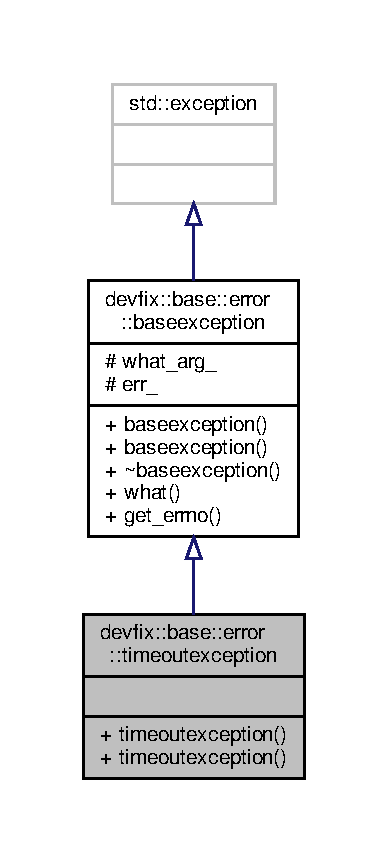
\includegraphics[width=186pt]{structdevfix_1_1base_1_1error_1_1timeoutexception__inherit__graph}
\end{center}
\end{figure}
\subsection*{Public Member Functions}
\begin{DoxyCompactItemize}
\item 
\hyperlink{structdevfix_1_1base_1_1error_1_1timeoutexception_a1795157a577b45e026b11c3b3cec80b3}{timeoutexception} (const std\+::string \&what\+\_\+arg, int err=0)
\item 
\hyperlink{structdevfix_1_1base_1_1error_1_1timeoutexception_ac35d347533a4a8ba1d19900846784e72}{timeoutexception} (const char $\ast$what\+\_\+arg, int err=0)
\end{DoxyCompactItemize}
\subsection*{Additional Inherited Members}


\subsection{Detailed Description}
Exception thrown when a blocking operation times out. 

Blocking operations for which a timeout is specified need a means to indicate that the timeout has occurred. For many such operations it is possible to return a value that indicates timeout; when that is not possible or desirable then Timeout\+Exception should be declared and thrown. 

\subsection{Constructor \& Destructor Documentation}
\mbox{\Hypertarget{structdevfix_1_1base_1_1error_1_1timeoutexception_a1795157a577b45e026b11c3b3cec80b3}\label{structdevfix_1_1base_1_1error_1_1timeoutexception_a1795157a577b45e026b11c3b3cec80b3}} 
\index{devfix\+::base\+::error\+::timeoutexception@{devfix\+::base\+::error\+::timeoutexception}!timeoutexception@{timeoutexception}}
\index{timeoutexception@{timeoutexception}!devfix\+::base\+::error\+::timeoutexception@{devfix\+::base\+::error\+::timeoutexception}}
\subsubsection{\texorpdfstring{timeoutexception()}{timeoutexception()}\hspace{0.1cm}{\footnotesize\ttfamily [1/2]}}
{\footnotesize\ttfamily devfix\+::base\+::error\+::timeoutexception\+::timeoutexception (\begin{DoxyParamCaption}\item[{const std\+::string \&}]{what\+\_\+arg,  }\item[{int}]{err = {\ttfamily 0} }\end{DoxyParamCaption})\hspace{0.3cm}{\ttfamily [inline]}, {\ttfamily [explicit]}}

Constructs the error object with what\+\_\+arg as explanatory string that can be accessed through \hyperlink{structdevfix_1_1base_1_1error_1_1baseexception_a16327152a55d65b1e537825231fbd452}{what()}. 
\begin{DoxyParams}{Parameters}
{\em what\+\_\+arg} & explanatory std\+::string \\
\hline
{\em err} & c error code (errno) \\
\hline
\end{DoxyParams}
\mbox{\Hypertarget{structdevfix_1_1base_1_1error_1_1timeoutexception_ac35d347533a4a8ba1d19900846784e72}\label{structdevfix_1_1base_1_1error_1_1timeoutexception_ac35d347533a4a8ba1d19900846784e72}} 
\index{devfix\+::base\+::error\+::timeoutexception@{devfix\+::base\+::error\+::timeoutexception}!timeoutexception@{timeoutexception}}
\index{timeoutexception@{timeoutexception}!devfix\+::base\+::error\+::timeoutexception@{devfix\+::base\+::error\+::timeoutexception}}
\subsubsection{\texorpdfstring{timeoutexception()}{timeoutexception()}\hspace{0.1cm}{\footnotesize\ttfamily [2/2]}}
{\footnotesize\ttfamily devfix\+::base\+::error\+::timeoutexception\+::timeoutexception (\begin{DoxyParamCaption}\item[{const char $\ast$}]{what\+\_\+arg,  }\item[{int}]{err = {\ttfamily 0} }\end{DoxyParamCaption})\hspace{0.3cm}{\ttfamily [inline]}, {\ttfamily [explicit]}}

Constructs the error object with what\+\_\+arg as explanatory string that can be accessed through \hyperlink{structdevfix_1_1base_1_1error_1_1baseexception_a16327152a55d65b1e537825231fbd452}{what()}. 
\begin{DoxyParams}{Parameters}
{\em what\+\_\+arg} & explanatory c-\/string \\
\hline
{\em err} & c error code (errno) \\
\hline
\end{DoxyParams}


The documentation for this struct was generated from the following file\+:\begin{DoxyCompactItemize}
\item 
devfix/base/error/\hyperlink{timeoutexception_8h}{timeoutexception.\+h}\end{DoxyCompactItemize}

%--- End generated contents ---

% Index
\backmatter
\newpage
\phantomsection
\clearemptydoublepage
\addcontentsline{toc}{chapter}{Index}
\printindex

\end{document}
